% Options for packages loaded elsewhere
\PassOptionsToPackage{unicode}{hyperref}
\PassOptionsToPackage{hyphens}{url}
\PassOptionsToPackage{dvipsnames,svgnames,x11names}{xcolor}
%
\documentclass[
  number]{elsarticle}

\usepackage{amsmath,amssymb}
\usepackage{iftex}
\ifPDFTeX
  \usepackage[T1]{fontenc}
  \usepackage[utf8]{inputenc}
  \usepackage{textcomp} % provide euro and other symbols
\else % if luatex or xetex
  \usepackage{unicode-math}
  \defaultfontfeatures{Scale=MatchLowercase}
  \defaultfontfeatures[\rmfamily]{Ligatures=TeX,Scale=1}
\fi
\usepackage{lmodern}
\ifPDFTeX\else  
    % xetex/luatex font selection
\fi
% Use upquote if available, for straight quotes in verbatim environments
\IfFileExists{upquote.sty}{\usepackage{upquote}}{}
\IfFileExists{microtype.sty}{% use microtype if available
  \usepackage[]{microtype}
  \UseMicrotypeSet[protrusion]{basicmath} % disable protrusion for tt fonts
}{}
\makeatletter
\@ifundefined{KOMAClassName}{% if non-KOMA class
  \IfFileExists{parskip.sty}{%
    \usepackage{parskip}
  }{% else
    \setlength{\parindent}{0pt}
    \setlength{\parskip}{6pt plus 2pt minus 1pt}}
}{% if KOMA class
  \KOMAoptions{parskip=half}}
\makeatother
\usepackage{xcolor}
\setlength{\emergencystretch}{3em} % prevent overfull lines
\setcounter{secnumdepth}{5}
% Make \paragraph and \subparagraph free-standing
\makeatletter
\ifx\paragraph\undefined\else
  \let\oldparagraph\paragraph
  \renewcommand{\paragraph}{
    \@ifstar
      \xxxParagraphStar
      \xxxParagraphNoStar
  }
  \newcommand{\xxxParagraphStar}[1]{\oldparagraph*{#1}\mbox{}}
  \newcommand{\xxxParagraphNoStar}[1]{\oldparagraph{#1}\mbox{}}
\fi
\ifx\subparagraph\undefined\else
  \let\oldsubparagraph\subparagraph
  \renewcommand{\subparagraph}{
    \@ifstar
      \xxxSubParagraphStar
      \xxxSubParagraphNoStar
  }
  \newcommand{\xxxSubParagraphStar}[1]{\oldsubparagraph*{#1}\mbox{}}
  \newcommand{\xxxSubParagraphNoStar}[1]{\oldsubparagraph{#1}\mbox{}}
\fi
\makeatother


\providecommand{\tightlist}{%
  \setlength{\itemsep}{0pt}\setlength{\parskip}{0pt}}\usepackage{longtable,booktabs,array}
\usepackage{calc} % for calculating minipage widths
% Correct order of tables after \paragraph or \subparagraph
\usepackage{etoolbox}
\makeatletter
\patchcmd\longtable{\par}{\if@noskipsec\mbox{}\fi\par}{}{}
\makeatother
% Allow footnotes in longtable head/foot
\IfFileExists{footnotehyper.sty}{\usepackage{footnotehyper}}{\usepackage{footnote}}
\makesavenoteenv{longtable}
\usepackage{graphicx}
\makeatletter
\newsavebox\pandoc@box
\newcommand*\pandocbounded[1]{% scales image to fit in text height/width
  \sbox\pandoc@box{#1}%
  \Gscale@div\@tempa{\textheight}{\dimexpr\ht\pandoc@box+\dp\pandoc@box\relax}%
  \Gscale@div\@tempb{\linewidth}{\wd\pandoc@box}%
  \ifdim\@tempb\p@<\@tempa\p@\let\@tempa\@tempb\fi% select the smaller of both
  \ifdim\@tempa\p@<\p@\scalebox{\@tempa}{\usebox\pandoc@box}%
  \else\usebox{\pandoc@box}%
  \fi%
}
% Set default figure placement to htbp
\def\fps@figure{htbp}
\makeatother

\makeatletter
\@ifpackageloaded{caption}{}{\usepackage{caption}}
\AtBeginDocument{%
\ifdefined\contentsname
  \renewcommand*\contentsname{Table of contents}
\else
  \newcommand\contentsname{Table of contents}
\fi
\ifdefined\listfigurename
  \renewcommand*\listfigurename{List of Figures}
\else
  \newcommand\listfigurename{List of Figures}
\fi
\ifdefined\listtablename
  \renewcommand*\listtablename{List of Tables}
\else
  \newcommand\listtablename{List of Tables}
\fi
\ifdefined\figurename
  \renewcommand*\figurename{Figure}
\else
  \newcommand\figurename{Figure}
\fi
\ifdefined\tablename
  \renewcommand*\tablename{Table}
\else
  \newcommand\tablename{Table}
\fi
}
\@ifpackageloaded{float}{}{\usepackage{float}}
\floatstyle{ruled}
\@ifundefined{c@chapter}{\newfloat{codelisting}{h}{lop}}{\newfloat{codelisting}{h}{lop}[chapter]}
\floatname{codelisting}{Listing}
\newcommand*\listoflistings{\listof{codelisting}{List of Listings}}
\makeatother
\makeatletter
\makeatother
\makeatletter
\@ifpackageloaded{caption}{}{\usepackage{caption}}
\@ifpackageloaded{subcaption}{}{\usepackage{subcaption}}
\makeatother

\usepackage[]{natbib}
\bibliographystyle{elsarticle-num}
\usepackage{bookmark}

\IfFileExists{xurl.sty}{\usepackage{xurl}}{} % add URL line breaks if available
\urlstyle{same} % disable monospaced font for URLs
\hypersetup{
  pdftitle={Draft -- Discriminating Seagrasses From Green Macroalgae in European Intertidal areas using high resolution multispectral drone imagery -- Draft},
  pdfauthor={Simon Oiry; Bede Ffinian Rowe Davies; Ana I. Sousa; Philippe Rosa; Maria Laura Zoffoli; Guillaume Brunier; Pierre Gernez; Laurent Barillé},
  pdfkeywords={Drone, Remote Sensing, Seagrass, Coastal
Ecosystems, Neural Network},
  colorlinks=true,
  linkcolor={blue},
  filecolor={Maroon},
  citecolor={Blue},
  urlcolor={Blue},
  pdfcreator={LaTeX via pandoc}}


\setlength{\parindent}{6pt}
\begin{document}

\begin{frontmatter}
\title{Draft -- Discriminating Seagrasses From Green Macroalgae in
European Intertidal areas using high resolution multispectral drone
imagery -- Draft}
\author[1]{Simon Oiry%
\corref{cor1}%
}
 \ead{oirysimon@gmail.com} 
\author[1]{Bede Ffinian Rowe Davies%
%
}

\author[2]{Ana I. Sousa%
%
}

\author[1]{Philippe Rosa%
%
}

\author[3]{Maria Laura Zoffoli%
%
}

\author[4]{Guillaume Brunier%
%
}

\author[1]{Pierre Gernez%
%
}

\author[1]{Laurent Barillé%
%
}


\affiliation[1]{organization={Institut des Substances et Organismes de
la Mer, ISOMer, Nantes Université, UR 2160, F-44000 Nantes,
France},,postcodesep={}}
\affiliation[2]{organization={ECOMARE - Laboratory for Innovation and
Sustainability of Marine Biological Resources, CESAM -- Centre for
Environmental and Marine Studies, Department of Biology, University of
Aveiro, Campus Universitário de Santiago, 3810-193 Aveiro,
Portugal},,postcodesep={}}
\affiliation[3]{organization={Consiglio Nazionale delle Ricerche,
Istituto di Scienze Marine (CNR-ISMAR), 00133 Rome,
Italy},,postcodesep={}}
\affiliation[4]{organization={BRGM French Geological Survey, Cayenne
97300, French Guiana},,postcodesep={}}

\cortext[cor1]{Corresponding author}








        
\begin{abstract}
Coastal areas support seagrass meadows, which offer crucial ecosystem
services including erosion control and carbon sequestration. However,
these areas are increasingly impacted by human activities, leading to
habitat fragmentation and seagrass decline. In situ surveys,
traditionally performed to monitor these ecosystems face limitations on
temporal and spatial coverage, particularly in intertidal zones,
prompting the addition of satellite data within monitoring programs.
Yet, satellite remote sensing can be limited by too coarse spatial
and/or spectral resolution, making it difficult to discriminate seagrass
from other macrophytes in highly heterogenous meadows. Drone (unmanned
aerial vehicles -- UAV) images at a very high spatial resolution offer a
promising solution to address challenges related to spatial
heterogeneity and intrapixel mixture. This study focuses on using drone
acquisitions with a ten spectral band sensor similar to that onboard
Sentinel-2, for mapping intertidal macrophytes at low tide (i.e.~during
a period of emersion) and effectively discriminating between seagrass
and green macroalgae. Nine drone flights were conducted at two different
altitudes (12 m and 120 m) across heterogeneous intertidal European
habitats in France and Portugal, providing multispectral reflectance
observation at very high spatial resolution (8 mm and 80 mm
respectively). Taking advantage of their extremly high spatial
resolution; the low altitude flights were used to train a Neural Network
classifier to discrimintate five taxonomic classes of intertidal
vegetation: Magnoliopsida (Seagrass), Chlorophyceae (Green macroalgae),
Phaeophyceae (Brown algae), Rhodophyceae (Red macroalgae) and benthic
Bacillariophyceae (Diatoms), and validated using concomitant field
measurements. Classification of drone imagery resulted in an overall
accuracy of 94\% across all sites and images, covering a total area of
467 000 m². The model exhibited an accuracy of 96.4\% in identifying
seagrass. In particular , seagrass and green algae can be discriminated.
The very high spatial resolution of the drone data made it possible to
assess the influence of spatial resolution on the classification
outputs, showing a limited loss in seagrass detection up to about 10m.
Altogether, out findings suggest that the Multi-Spectral Instrument
(MSI) onboard Sentinel-2 offers a relevant trade-off between its spatial
and spectral resolution, thus offering promising perspectives for
satellite remote sensing of intertidal biodiversity over lager scales.
\end{abstract}





\begin{keyword}
    Drone \sep Remote Sensing \sep Seagrass \sep Coastal
Ecosystems \sep 
    Neural Network
\end{keyword}
\end{frontmatter}
    

\section{Introduction}\label{introduction}

Coastal areas are vital hotspots for marine biodiversity, with
intertidal seagrass meadows playing a crucial role at the interface
between land and ocean \citep{unsworth2022}. Seagrass meadows provide a
myriad of ecosystem services, including carbon sequestration, oxygen
production, protection against sea-level rise and coastline erosion, and
mitigation of eutrophication \citep{unsworth2022, sousa2019blue}. They
serve as vital habitats for a diverse array of marine and terrestrial
species, providing living, breeding, and feeding grounds
\citep{gardner2018, Zoffoli2022, jankowska2019}. Due to the
concentration of human activities in coastal zones, seagrass meadows are
directly exposed to and impacted by anthropogenic pressures. Global
regression and fragmentation of seagrass meadows are currently observed
due to climate change, diseases, urbanization, land reclamation,
dredging, competition with alien species, and reduction in water quality
\citep{nguyen2021, soissons2018, orth2006, lin2018, duffy2019, rasheed2011long, chefaoui2018dramatic, sousa2019blue}.
Both habitat fragmentation and reduction, in turn, can severely
compromise the effectiveness of ecosystem services provided by seagrass
meadows. While improvements in water quality and hydrodynamics have been
recently reported in Europe, allowing an overall recovery of seagrass
ecosystems at local and European scales, many coastal waters worldwide
are still subjected to strong eutrophication processes
\citep{deSantos2019, Zoffoli2021, sousa2019blue}. Coastal eutrophication
has been associated to excessive accumulation of green macroalgae,
so-called green tides \citep{devlin2023nutrients}. Green tides produce
shade and suffocation over seagrass individuals, thus threatening the
health of seagrass ecosystems \citep{wang2022}.

The importance of seagrass meadows and the variety of ecosystem services
they provide have led to the enhancement of both global and regional
programs to monitor Essential Oceanic Variable (EOVs) such as seagrass
composition \citep{Miloslavich2018}, as well as Essential Biodiversity
Variable (EBVs) such as seagrass taxonomic diversity, species
distribution, population abundance, and phenology \citep{Pereira2013}.
Traditionally, indicators of seagrass status have been quantified using
\emph{in situ} measurements. However, the acquisition of field
measurements in intertidal zones is notoriously challenging. Intertidal
seagrass meadows are only exposed during low tide and can be situated in
difficult-to-reach mudflats, potentially leading to inaccurate and
limited estimations with conventional sampling techniques
\citep{nijland2019}. Satellite observations have been proven effective
in complementing \emph{in situ} sampling, allowing for near real-time
and consistent retrieval of seagrass EOVs and EBVs over extensive
meadows
\citep{Zoffoli2021, xu2021, Traganos2018, coffer2023, davies2024intertidal, davies2024sentinel}.

While satellite remote sensing (RS) provides temporally consistent
observations over large spatial scales, its utilization over intertidal
areas is limited by several constraints. Satellite missions with a high
temporal resolution (e.g.~daily MODIS observation) are limited by too
coarse spatial resolution (\textgreater100 m) to accurately map patchy
seagrass meadows. Missions with a high spatial resolution such as
Sentinel-2 (10 m) or Landsat8/9 (30 m) can be limited by low spectral
resolution. The limited number of spectral bands challenges accurate
discrimination of seagrass from other co-existing macrophytes. In
particular, Chlorophyceae (green algae) and marine Magnoliopsida
(seagrass) share the same pigment composition
\citep{ralph2002, Douay2022}, resulting in a similar spectral signature
in terms of reflectance, especially in the visible range
\citep{Davies2023, bannari2022}. Recently, using advanced
machine-learning algorithms trained with a large hyperspectral library
of more than 300 field reflectance spectra, \citep{Davies2023}
demonstrated that it was possible to discriminate Magnoliopsida from
Chlorophyceae using reflectance spectra at Sentinel-2 's spectral
resolution. However the application of this approach to satellite RS
remains to be validated. Moreover patches of green algae can develop at
small spatial scales that are not observable using Sentinel-2 and/or
Landsat-8/9 images \citep{tuya2013}, especially during the initial stage
of a green tide.

Drones (Unmanned Aerial Vehicles -- UAVs) can potentially fill the data
gaps left by satellite RS and \emph{in situ} measurements, due to their
ability to provide spatially-explicit observations at very high spatial
resolutions (pixel size from mm to cm) while capturing data at
multi-spectral resolution \citep{fairley2022drone, oh2017use}. The
versatility of drones allows for their application across a diverse
thematic range , from coastal zone management
\citep{adade2021, casella2020, angnuureng2022} to mapping species
distribution
\citep{joyce2023, tallam2023, Roca2022, Roman2021, Brunier2022Topographic, sousa2019blue}.
However, when applied to coastal habitat mapping, previous case studies
were mostly limited to a low number of \textbf{drone} flights over a
single study site, restricting the generalizability of their application
over wider geographical scales
\citep{Roman2021, collin2019improving, rossiter2020uav, Brunier2022Topographic}.
\textbf{These studies have demonstrated the capability of drones to map
intertidal habitats, including seagrasses; however, broader
generalization of these findings is still lacking. The current paper
uniquely expands the spatial and methodological scope of drone-based
remote sensing for intertidal habitat mapping across a broad
biogeographical range. It demonstrates the feasibility of accurately
classifying diverse macrophyte types across various study sites, with a
particular focus on distinguishing Magnoliopsida (seagrasses) and
Chlorophyceae (green algae). Unlike previous studies, our approach
integrates multiple spatial scales by simulating satellite resolutions
and quantifying the impact of spatial resolution on classification
accuracy.} Nine drone flights were performed over soft-bottom intertidal
areas along the Atlantic coastlines of two European countries (France
and Portugal), covering a wide range of habitats, from monospecific
seagrass meadows to meadows mixed with green, or red macroalgae. A deep
learning algorithm was trained and validated for macrophyte
discrimination, emphasizing applicability across diverse sites without a
loss of prediction accuracy. The classification maps obtained at a very
high spatial resolution with the drone were spatially degraded to
satellite resolutions, making it possible to assess the effect of
spatial resolution on classification accuracy, and provide insights for
coastal habitat mapping using satellite remote sensing. \textbf{This
study is, therefore, among the first to quantify the effects of spatial
resolution on the accuracy of drone-based macrophyte classification
across a wide geographical scale, providing a framework for to better
understand satellite-based classification challenges.}

\section{Material \& Methods}\label{material-methods}

\subsection{Study sites}\label{study-sites}

Seven study sites distributed between France and Portugal were selected
for their extensive intertidal seagrass beds. Two sites were located in
the Gulf of Morbihan, France (Figure~\ref{fig-map} A : 47.5791°N,
2.8018°W). This gulf covers an area of 115 km² and is only connected to
the sea through a 900 m wide channel. A total of 53 small islands are
scattered across the gulf leading to 250 km of shorelines. Patchy
seagrass meadows can be found on many of these islands. One of the sites
within the gulf was on one its islands (Arz) and the other was located
further south on a mainland beach area (Duer). The Gulf of Morbihan is a
Natura 2000 site and a Regional Protected Area due to its rich
biodiversity, including its seagrass meadows, and is also classified as
a RAMSAR site, which highlights its significance as a wetland of
international importance. Two other sites were located in Bourgneuf Bay,
France (Figure~\ref{fig-map} B : 46.9849°N, 2.1488°W) which is a 340 km²
semi-enclosed macrotidal bay, protected from waves by Noirmoutier
Island. Bourgneuf bay hosts a large intertidal seagrass meadow of about
6 km² \citep{ZOFFOLI2020112020}. Within this meadow, the sites observed
by drones (L'Epine and Barbatre) contained monospecific beds of
\emph{Zostera noltei} (dwarf eelgrass) with very little mixing with
other macrophytes. Bourgneuf Bay is also part of the Natura 2000 network
and serves as a RAMSAR site due to its critical habitat for migratory
bird species and its extensive seagrass meadows \citep{Zoffoli2022}.
Three sites were surveyed in the Ria de Aveiro Coastal Lagoon in
Portugal (Figure~\ref{fig-map} C : 40.6887°N, 8.6810°W). The extent of
this lagoon is \textasciitilde83 km² (at low tide) with many narrow
channels, large salt marshes and many mudflats that uncover at low tide
\citep{sousa2017blue}. It is connected to the open sea through a single
channel, with a tidal lag between the North and the South of the lagoon.
The southernmost site (Gafanha) is a mudflat located in the Mira channel
(one of the four main channels of the lagoon) whereas the two other
sites (Mataducos and Marinha Lanzarote) were situated in the middle of
the lagoon and only accessible by boat. These Portuguese sites are
characterized by a more diverse intertidal vegetation, where patches of
seagrass intermingle with red, brown, and green macroalgae. The Aveiro
Lagoon, like the other study areas, is a Natura 2000 site and a RAMSAR
wetland, recognized for its rich mosaic of habitats and importance for
biodiversity, including migratory bird species and intertidal
vegetation.

\phantomsection\label{cell-fig-map}
\begin{figure}[H]

\centering{

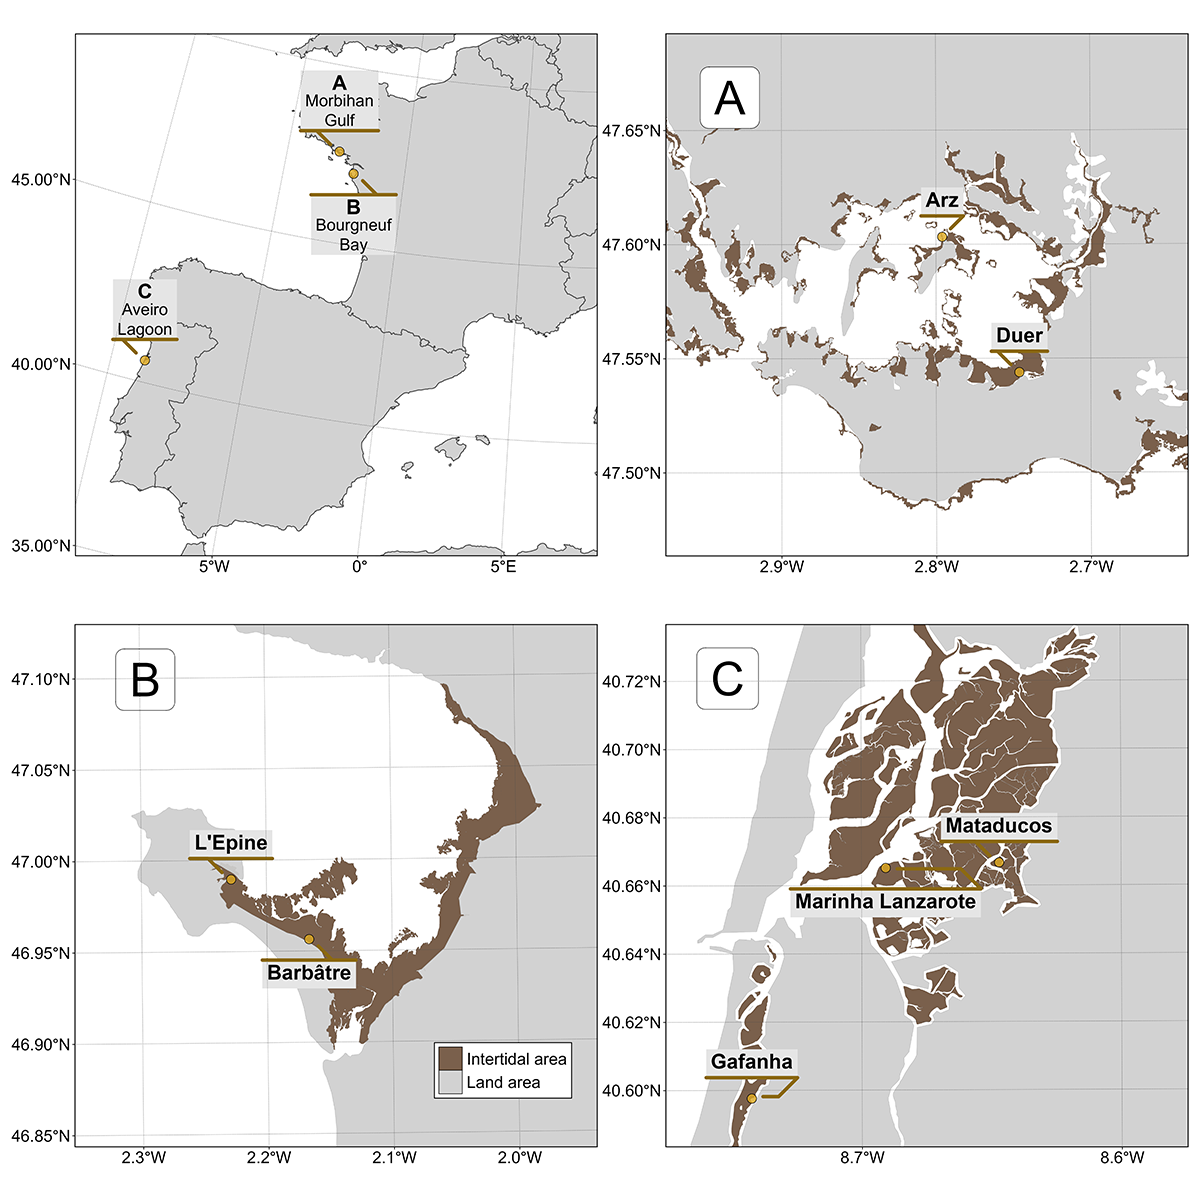
\includegraphics[width=1\linewidth,height=\textheight,keepaspectratio]{./Figures/Low_res/Fig1_Map_Drone_Sites.png}

}

\caption{\label{fig-map}Location of drone flights in France and
Portugal. A: Gulf of Morbihan (Two sites), B: Bourngeuf Bay (Two sites),
C: Ria de Aveiro Coastal Lagoon (Three sites). Green areas represents
the intertidal zone.}

\end{figure}%

\subsection{Field sampling}\label{field-sampling}

\subsubsection{Drone acquisition}\label{drone-acquisition}

At each location, a DJI Matrice 200 quadcopter drone equipped with a
Micasense RedEdge Dual MX multispectral camera was flown to take 1.2
million pixel reflectance photographs with ten spectral bands ranging
from the blue to the near infrared (NIR): 444, 475, 531, 560, 650, 668,
705, 717, 740 and 840 nm. To ensure consistent lighting conditions
across flight paths, the drone's trajectory was aligned to maintain a
solar azimuth angle of 90 degrees. An overlap of 70\% and 80\% (side and
front respectively) between each image was set for each flight. A
downwelling light sensor (DLS2) was used to acquire irradiance data
concomitantly with the camera measurements. Raw data were calibrated in
reflectance using a calibration panel reflective at \textasciitilde50\%
provided by the manufacturer. Across all sites, flights were made at two
different altitudes : 12 m or/and 120 m, with a spatial resolution of 8
mm and 80 mm, respectively (Table~\ref{tbl-flights}). \textbf{Low
altitude flights were used as training dataset for a neural network
model while high altitude flight were used for validation.}

\begin{table}

\caption{\label{tbl-flights}List of drone flight, summarising the date,
the altitude, and the purpose of each flight. 12 m and 120 m flights
have a spatial resolution of 8 and 80 mm respectively.}

\centering{

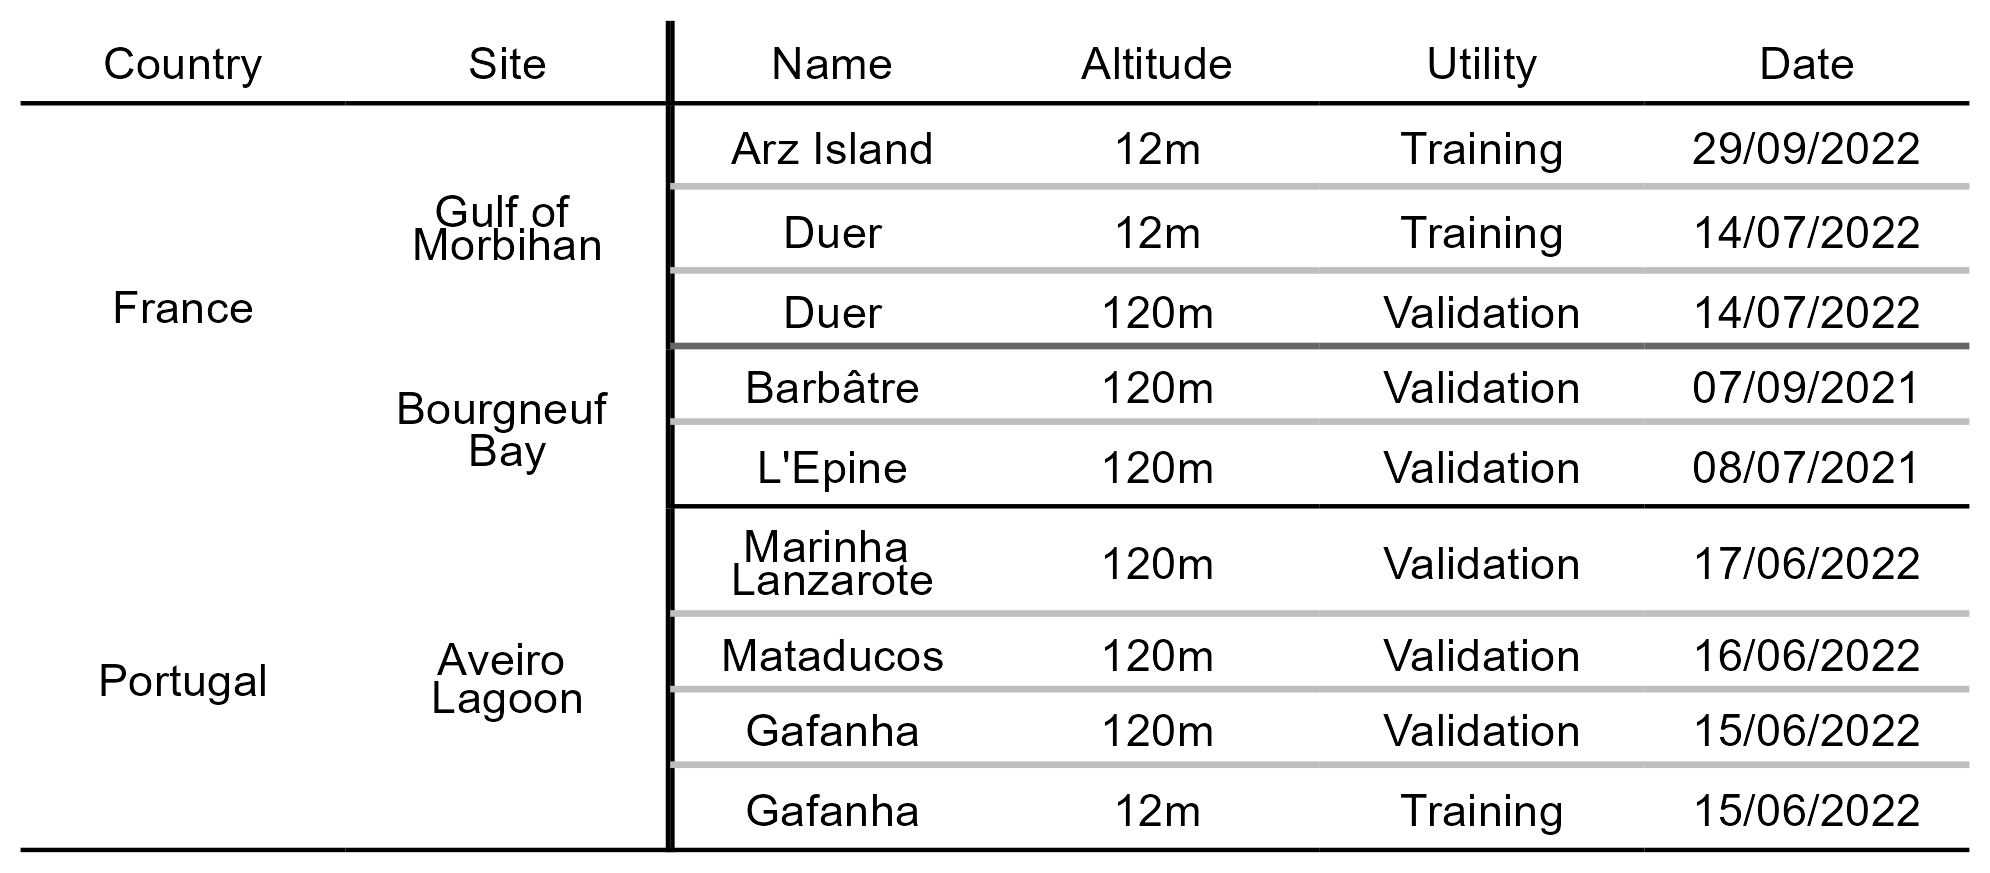
\includegraphics[width=6.63in,height=\textheight,keepaspectratio]{Figures/High_res/Table1/table_flights.png}

}

\end{table}%

\subsubsection{Ground Control Points}\label{ground-control-points}

Before each flight, targets used as ground control points were
distributed over the study site and georeferenced with a Trimble © Geo
XH 6000 differential GPS (dGPS). Ground control points were used to
correct georeferencing imprecision of orthomosaics with an horizontal
and vertical accuracy of 10cm. A dGPS was also used to georeference
quadrats of 0.25 m² ,which assessed the presence or absence of five key
taxonomic classes of intertidal vegetation : Bacillariophyceae
(unicellular benthic diatoms forming biofilms at the sediment surface
during low tide, \textbf{ranging in size from small patches (m²) to
entire mudflats (km²)}; henceforth: Diatoms), Phaeophyceae (henceforth:
brown macroalgae), Magnoliopsida (henceforth: Seagrasses), Chlorophyceae
(henceforth: Green macroalgae) and Rhodophyceae (henceforth: red
macroalgae) (Figure~\ref{fig-vegetation}). Only homogeneous vegetation
patches extending over several meters were selected as ground control
points. Pictures of each quadrat were uploaded online to the open-portal
Global Biodiversity Information Facility (GBIF) platform
\citep{BedeGbif}. Each photograph was also processed to estimate the
percent cover of each type of vegetation using an image processing
software \citep[ImageJ,][]{schneider2012nih}. Hyperspectral reflectance
signatures of each vegetation class were recorded using an ASD FieldSpec
HandHeld 2 spectroradiometer, which acquires reflectance between 325 and
1075 nm, with 1 nm of spectral resolution. Hyperspectral signatures
served dual purposes: they validate the radiometric calibration of drone
data and contribute to misclassification reduction in photo
interpretations.

\phantomsection\label{cell-fig-vegetation}
\begin{figure}[H]

\centering{

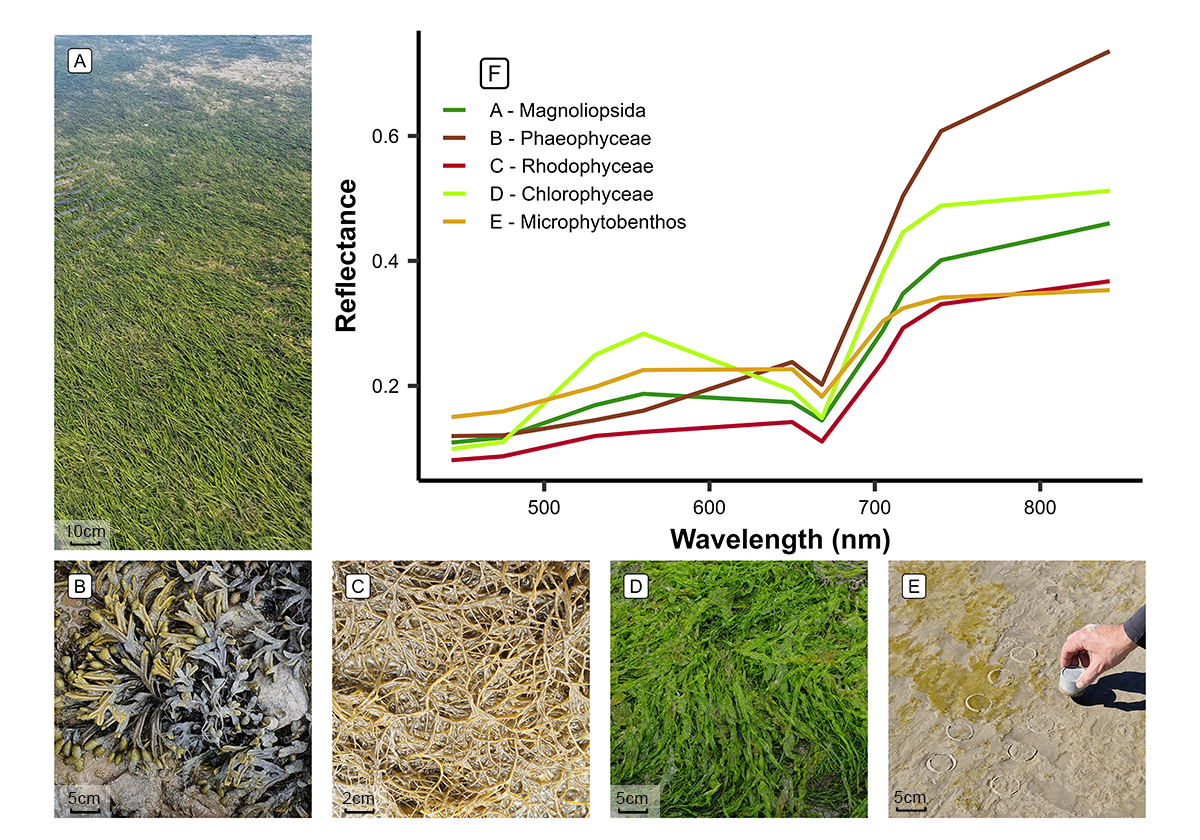
\includegraphics[width=1\linewidth,height=\textheight,keepaspectratio]{Figures/Low_res/Spectral_shapes_total.png}

}

\caption{\label{fig-vegetation}The five taxonomic classes of vegetation
used to train the Neural Network model and an example of their raw
spectral signatures at the spectral resolution of the Micasense RedEdge
Dual MX. A : Magnoliopsida (\emph{Zostera noltei}) ; B : Phaeophyceae
(\emph{Fucus sp.}) ; C : Rhodophyceae (\emph{Gracilaria
vermiculophylla}) ; D : Chlorophyceae (\emph{Ulva sp.}) ; E :
Bacillariophyceae (Diatoms - MPB). \textbf{Classes were identified
following the World register of Marine species.}}

\end{figure}%

\subsection{Drone Processing}\label{drone-processing}

A structure-from-motion photogrammetry software \citep[Agisoft
Metashape,][]{agisoft} was used to process images to obtain
multispectral orthomosaics of each flight. The process for
orthomosaicking was identical for every flight. First, key tying points
were detected inside of each image and between overlapping images in
order to obtain a sparse point cloud. This cloud was cleaned using a
reprojection accuracy metric in order to remove noisy points. A dense
point cloud was then produced using a structure from motion algorithm. A
surface interpolation of this dense point cloud was made to obtain a
digital surface model (DSM), used to reconstruct the multispectral
ortho-image \citep{nebel2020review}. Low altitude drone flights produced
ortho-images with a very high spatial resolution (8 mm per pixel),
making it efficient to visually distinguish between the various types of
vegetation. High altitude flights allowed to cover larger areas and
produced images with a pixel size of 80 mm (Table~\ref{tbl-flights}).

\subsection{General Workflow}\label{general-workflow}

The spectral similarities of the reflectance signatures at the spectral
resolution of the micasense senor between intertidal green macrophytes
(Magnoliopsida and Chlorophyceae) make their discrimination challenging
using simple classification algorithms (Figure~\ref{fig-vegetation} F).
To overcome this challenge, a deep learning classification method was
trained, validated, and applied to each drone flight
(Figure~\ref{fig-workflow}).

\phantomsection\label{cell-fig-workflow}
\begin{figure}[H]

\centering{

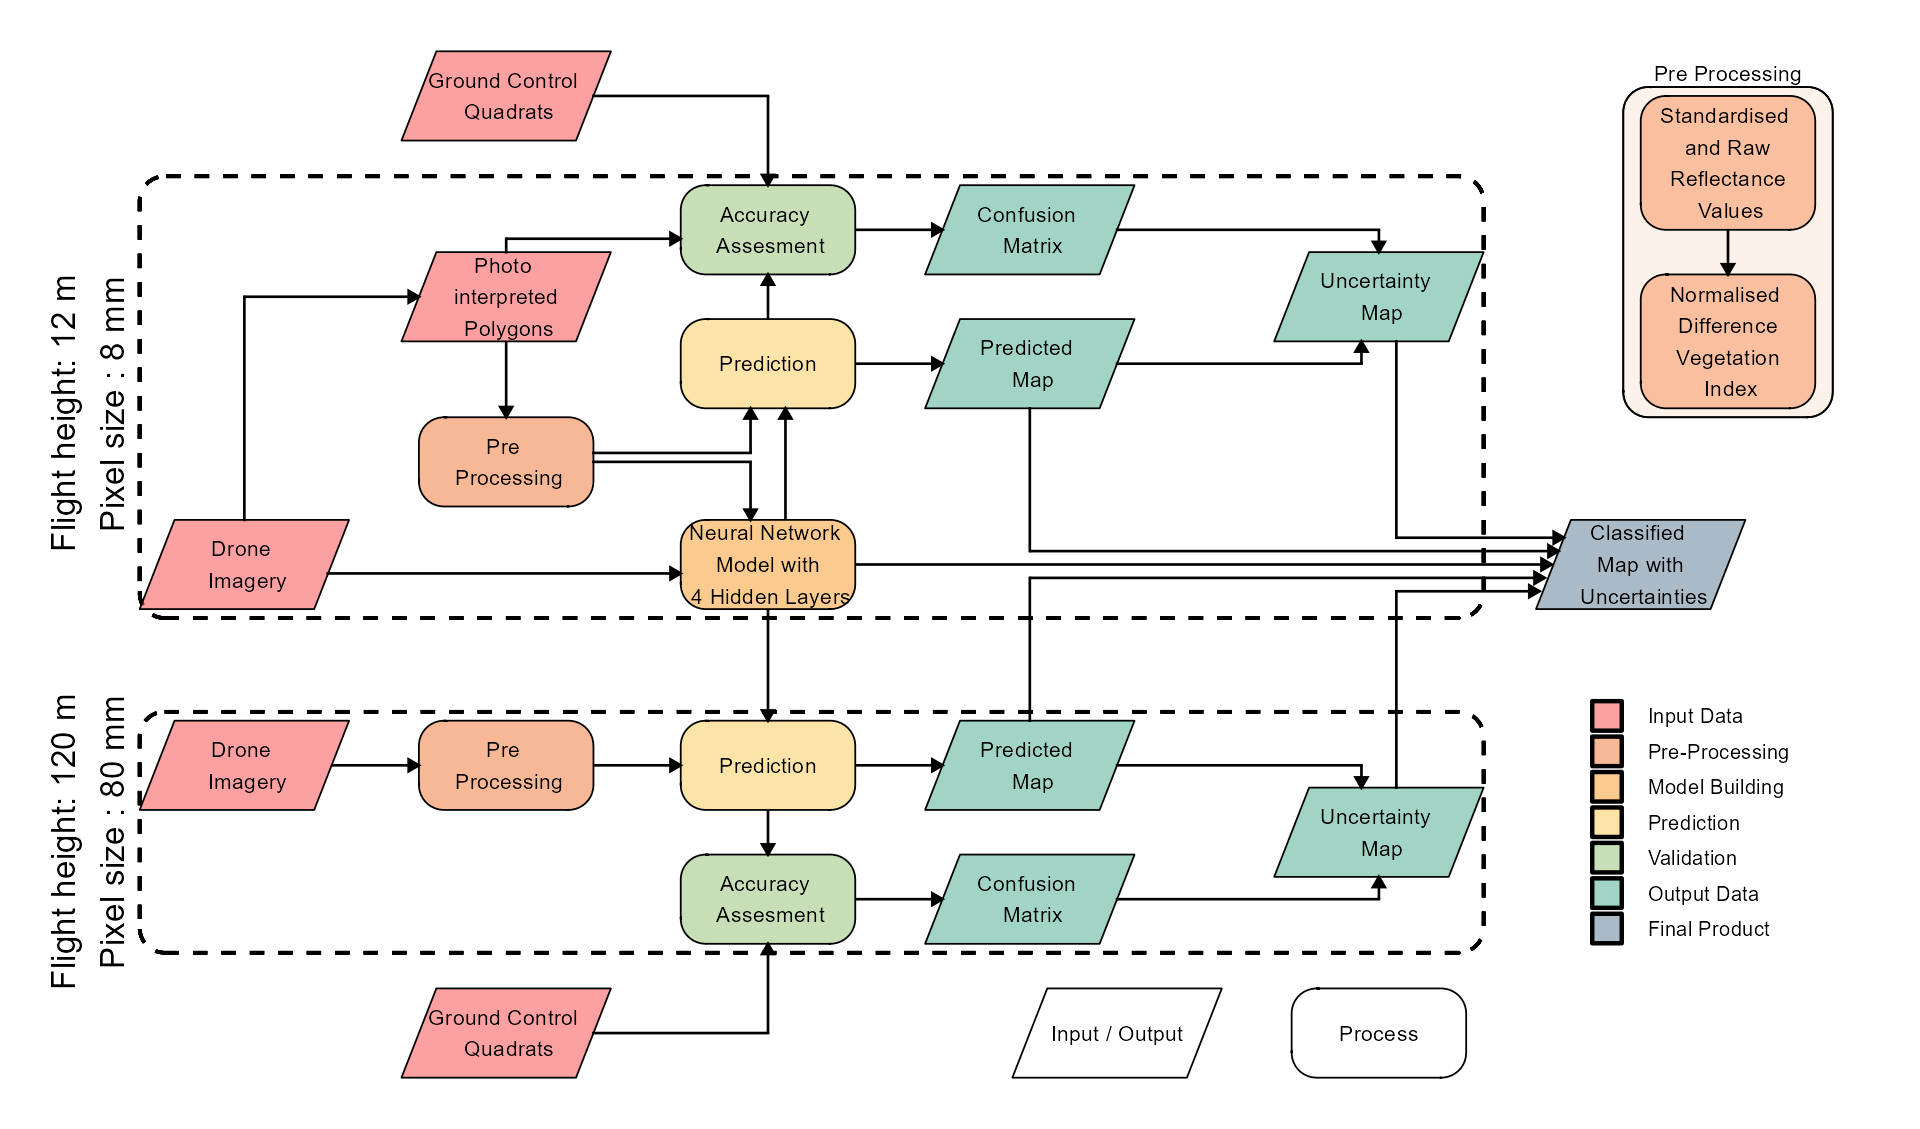
\includegraphics[width=1\linewidth,height=\textheight,keepaspectratio]{./Figures/Low_res/Figure3_workflow.png}

}

\caption{\label{fig-workflow}Schematic representation of the workflow.
Parallelograms represent input or output data, and rectangles represent
Python processing algorithms. The overall workflow of this study is
divided into two distinct parts based on the spatial resolution of the
drone flights: high-resolution flights (pixel size: 8 mm) were utilized
for training and prediction of the Neural Network model, whereas
lower-resolution flights (pixel size: 80 mm) were solely employed for
prediction purposes. Validation has been performed on both high and low
resolution flights.}

\end{figure}%

\subsubsection{Training dataset
building}\label{training-dataset-building}

\begin{table}

\caption{\label{tbl-validationPX}Vegetation Classes of the model and the
number of pixels used to train and validate each class}

\centering{

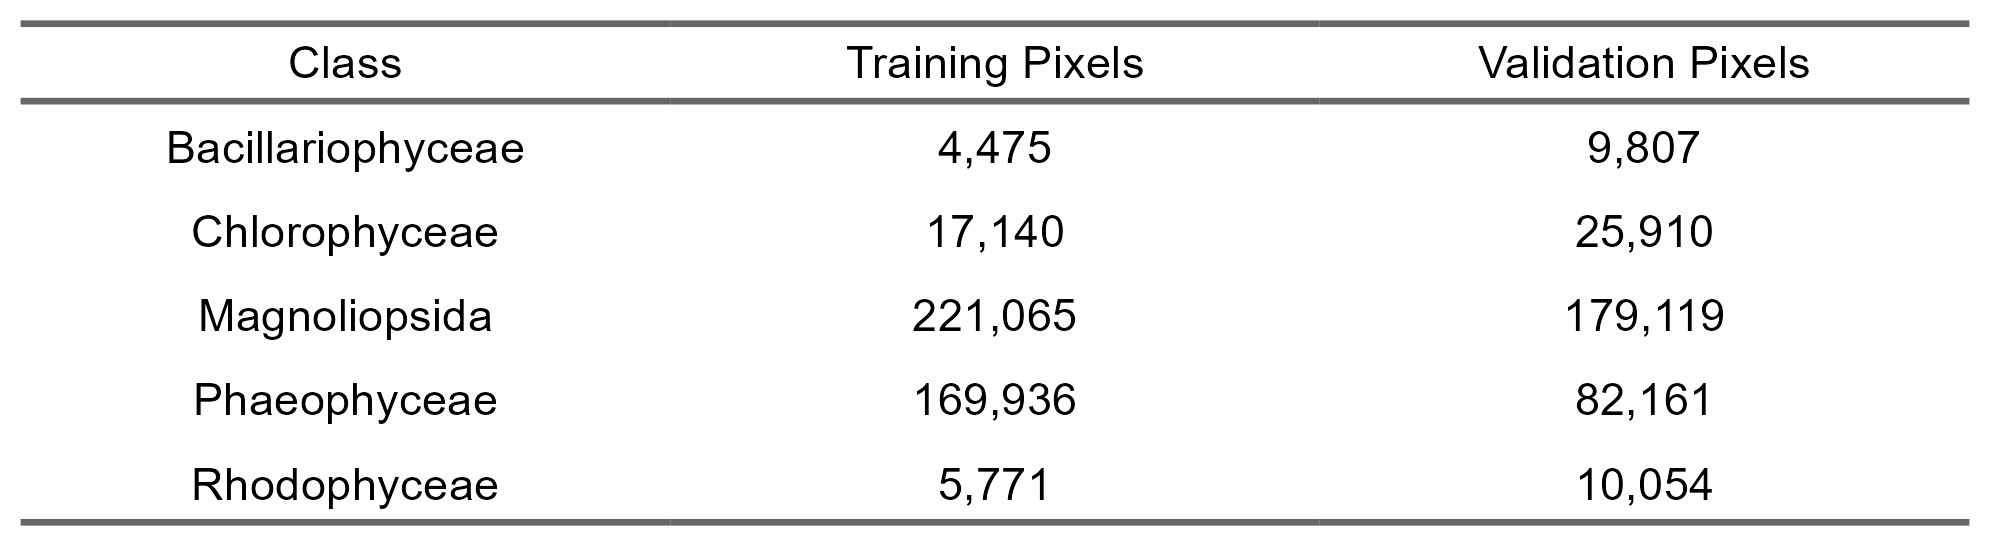
\includegraphics[width=6.63in,height=\textheight,keepaspectratio]{Figures/High_res/table_validation_px.png}

}

\end{table}%

A dataset containing photo-interpreted drone reflectance pixels was
built to train a Neural Network model. The training pixels were
categorized into seven different classes, representing the various
habitats encountered at the different study sites: Sediment, Water,
green macroalgae, seagrasses, diatoms, brown macroalgae and red
macroalgae. Only data from the low-altitude flights
(Table~\ref{tbl-flights}) were used for training because their 8 mm
spatial resolution allowed to avoid spectral sub-pixel mixing and to
accurately identify vegetation classes. \textbf{In the field, seagrasses
displaying two distinct colors, each with a unique spectral signature,
were observed. Careful attention was given to incorporating training
pixels from both color types into the training dataset for the seagrass
class. This approach was consistently applied to all classes within the
model.} More than 418,000 pixels at 8 mm resolution from the 3 training
flights were used to train the model (Table~\ref{tbl-validationPX}).
Twenty one variables were used by the model as predictors: the ten raw
spectral bands of the Micasense RedEdge Dual MX multispectral camera
(ranging from 444 nm to 840 nm), the same ten spectral bands
standardized using a min/max transformation (Equation~\ref{eq-std} ;
\citep{Cao2017}) and the Normalized difference vegetation index (NDVI,
Equation~\ref{eq-ndvi}). Standardisation of spectral bands is commonly
used to eliminate the scaling differences between spectra and to limit
the effect of biomass on the spectra shape
\citep{Douay2022, Davies2023}.

\begin{equation}\phantomsection\label{eq-std}{
R_{i}^{*}(\lambda) = \frac{R_{i}(\lambda) - min(R_{i})}{max(R_{i})- min(R_{i})}
}\end{equation}

where \(R_{i}(\lambda)\) is the reflectance at the wavelength
\((\lambda)\) of each individual spectra \((i)\), \(min(R_{i})\), and
\(max(R_{i})\) are the minimum and maximum value of the spectra \((i)\)

\begin{equation}\phantomsection\label{eq-ndvi}{
NDVI = \frac{R(840nm)-R(668nm)}{R(840nm)+R(668nm)}
}\end{equation}

where \(R(840nm)\) is the reflectance at 840 nm and \(R(668nm)\) is the
reflectance at 668 nm.

\subsubsection{Model building}\label{model-building}

A neural network classification model was built using the fastai
workflow \citep{howard2018fastai}. This model was composed of 2 hidden
layers and have a total of 26 054 trainable parameters. Parameters have
been fine tuned using 12 epoch to minimize the error rate. This model
has been called DISCOV, standing for Drone Intertidal Substrat
Classification Of Vegetation.

\subsubsection{Validation}\label{validation}

The workflow of this study revolves around two distinct flight heights
(12 and 120 m, Figure~\ref{fig-workflow}) where ensuring consistency
between reflectances at both heights is crucial. This comparison was
conducted at sites where low and high altitude flights overlapped. The
low altitude flights were resampled to the same spatial resolution and
grid as the high flights using a median resampling method. Reflectance
values were then extracted, and a scatterplot was generated and the Root
Mean Square Error (RMSE) was computed to compare the difference bewteen
the raw and standardised reflectance.

The classification model was applied to all flights at both 12 and 120 m
of altitude. \emph{In situ} information on georeferenced class type and
percent cover, acquired over homogeneous vegetation patches at the same
time as drone flights was used to assess the model accuracy. These
images were used to construct a validation dataset indicating the
presence or absence of each class. Additionally to the quadrat-based
validation dataset, polygons of each class were photo interpreted in
order to increase the number of pixels of the validation dataset. A
total of 536,000 pixels were used to validate the Neural Network
classifier. The sites with the lowest and highest number of validation
data were Gafanha Low (17316 pixels) and Marinha Lanzarote (159713
pixels), respectively. A confusion matrix, along with precision metrics
such as global accuracy, sensitivity, specificity, F1 score, and Kappa
coefficient, were generated for each site. These metrics were computed
as follow :

\[
\text{Global accuracy} = \frac{\sum_{i=1}^{k} \text{TP}_i}{\sum_{i=1}^{k} \left(\text{TP}_i + \text{FP}_i + \text{FN}_i \right)}
\] \[
\text{Sensitivity}_i = \frac{\text{TP}_i}{\text{TP}_i + \text{FN}_i}
\] \[
\text{Specificity}_i = \frac{\text{TN}_i}{\text{TN}_i + \text{FP}_i}
\] \[
\text{F1}_i = \frac{2 \cdot \text{TP}_i}{2 \cdot \text{TP}_i + \text{FP}_i + \text{FN}_i}
\] Where \(\text{TP}_i\), \(\text{TN}_i\), \(\text{FN}_i\) and
\(\text{FP}_i\) represent the true positives, true negatives, false
negatives and false positives relative to the class i.

All validation matrices were then aggregated to create an overall matrix

\subsection{Variable Importance}\label{variable-importance}

Variable Importance Plots (VIP) serve as a method to identify which
predictors are important for predicting a specific class. Out of the 21
predictors utilized in this study, Variable Importance was computed only
for the raw and standardized values of the 10 spectral bands captured by
the MicaSense camera. This is achieved by repeatedly predicting the same
dataset while randomly shuffling one predictor at a time. The benchmark
score obtained after each iteration is then compared to the benchmark
score obtained without shuffling any variables. The greater the
difference between these two benchmark values, the more important the
variable is for the model \citep{WEI2015399}.

\subsection{Influence of the spatial resolution on
classification}\label{influence-of-the-spatial-resolution-on-classification}

To assess the impact of spatial resolution on the model's output, we
resampled the drone orthomosaics from their native resolution (8 cm for
high-altitude flights) using the ``average'' method from the terra
package in R. \textbf{The rasters were resampled to 32 different
resolutions, ranging from 10 cm to 30 m.} DISCOV was then applied to
these resampled rasters, and the results were compared to the original
model predictions. For each resolution and vegetation class, we
calculated the predicted area loss, where a score of 0 indicates no area
loss during spatial resampling, and a score of 100 indicates complete
loss of the vegetation class.

We used a Generalized Linear Model (GLM) with a Beta distribution to
examine the relationship between pixel resolution, vegetation class, and
their interaction on the loss of vegetation. The loss of vegetation was
modelled as function of the interaction between pixel resolution and
vegetation class (Diatoms, brown macroalgae, seagrass, green macroalgae
and red macroalage). Sample vs fitted residuals and quartile-quartile
graphics were assessed visually, to ensure assumption of the models used
were met.

\subsection{Impact of mixed vegetation cover on the
prediction}\label{impact-of-mixed-vegetation-cover-on-the-prediction}

The key aspect of the workflow adopted in the present study is the
mapping at two different altitudes (12 and 120 m), resulting in two
distinct resolutions for the same area (8 and 80 mm; respectively). The
high-resolution flight was used to estimate the sub-pixel composition
for each pixel of the lower-resolution flight. Consequently, within each
pixel of the high-altitude flights, the contribution of each vegetation
class (\% cover) was obtained, and a kernel density plot was generated.
This plot provided a visual representation of the model's behavior in
mixed vegetation scenarios. It helps to understand the minimum
vegetation cover of a given class within a pixel necessary for the model
to confidently predict that class.

\section{Results}\label{results}

\subsection{Reflectance comparison between the two different
altitudes}\label{reflectance-comparison-between-the-two-different-altitudes}

In this study, drone flights were conducted at two different altitudes
(12 and 120 m) to construct the neural network model. At the sites where
the flights at both altitudes overlapped, reflectance was compared.
Overall there was a good agreement between the two altitudes (RMSE :
0.027 ; Figure~\ref{fig-CompareRef}).

\phantomsection\label{cell-fig-CompareRef}
\begin{figure}[H]

\centering{

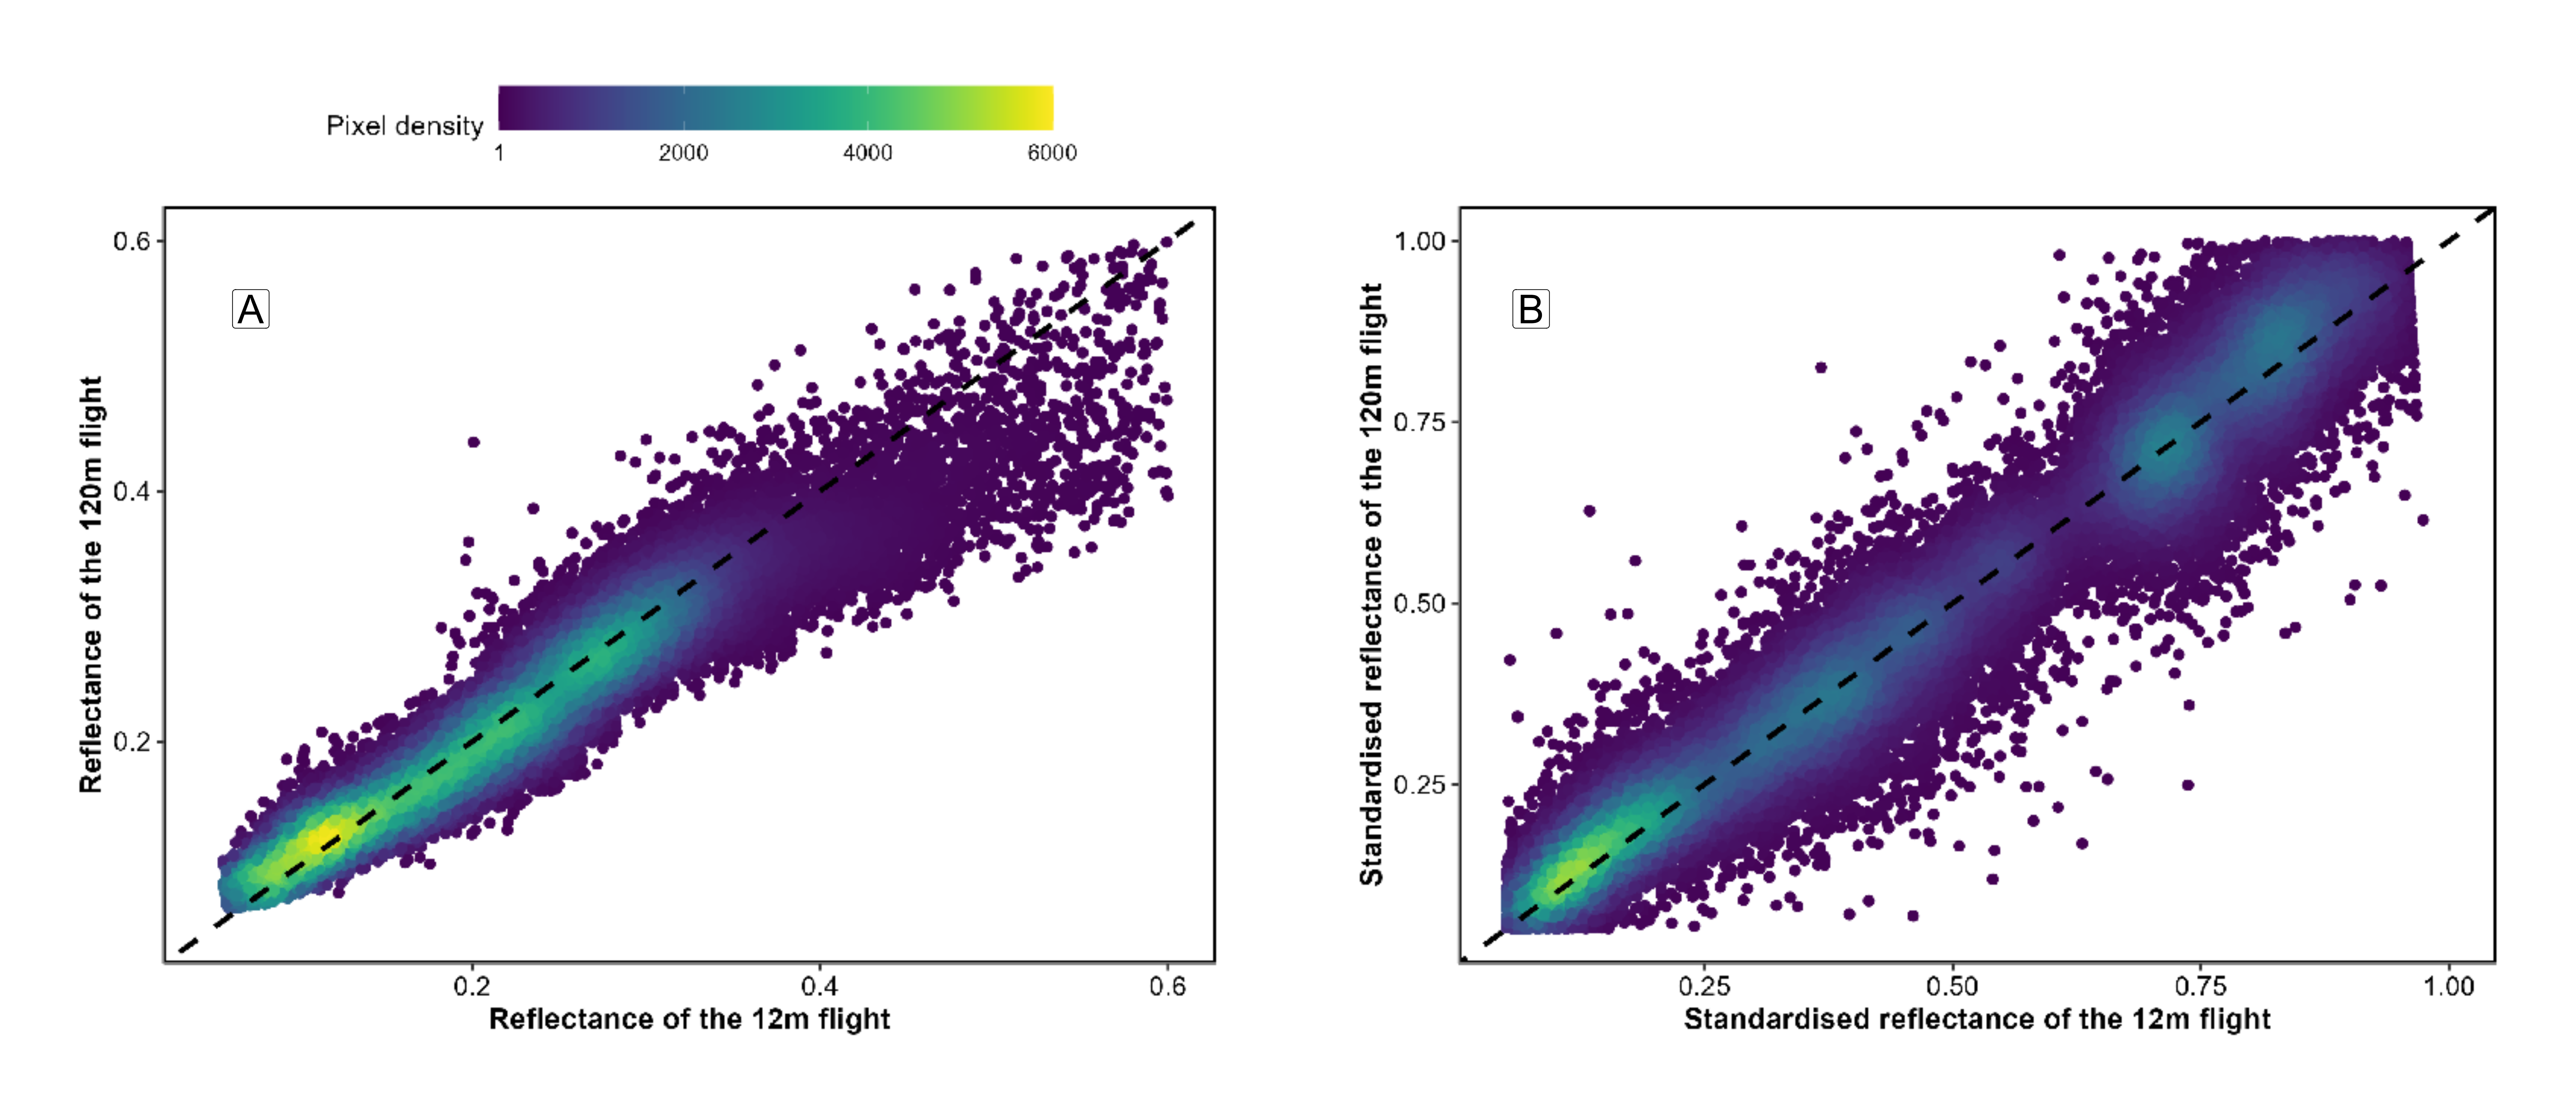
\includegraphics[width=1\linewidth,height=\textheight,keepaspectratio]{./Figures/High_res/Compare_reflectance_both.png}

}

\caption{\label{fig-CompareRef}Comparison of reflectance retrieved from
both low-altitude and high-altitude flights over a common area. The
black dashed line represents a 1 to 1 relationship. Left (A) plots raw
data and right (B) plots standardized data (Equation~\ref{eq-std}).}

\end{figure}%

There was a slight underestimation for raw reflectance values in the
high-altitude flight, particularly for higher reflectance values
(Figure~\ref{fig-CompareRef} A). Since both flights were conducted over
vegetated areas, the highest reflectance values correspond to the
infrared part of the spectrum. This difference was not present when the
reflectance has been standardized (Equation~\ref{eq-std} ;
Figure~\ref{fig-CompareRef} B).

\subsection{Classification}\label{classification}

Each drone flight was used to produce a prediction map, as well as a
probability map that indicates the model derived probability of the
selected class for every pixel. The low-altitude flight conducted in
Gafanha, Portugal, represented the site with the highest complexity
(Figure~\ref{fig-GafLow}). Among the five vegetation classes on which
the model was trained, four were present on this site, with green and
red macroalgae mixed with a seagrass meadow. There was also diatoms
forming biofilms on bare sediment surface. Although the seagrass was
solely composed of a single specie, \emph{Zostera noltei}, various
colors of this specie could be observed from dark green (corresponding
to healthy leaves) to brown (when leaves are senescent or have an
altered pigment composition). Regardless of the variation of color, the
class Magnoliopsida (seagrass) was accurately predicted by the model (F1
score of 0.96 at that site).

\phantomsection\label{cell-fig-GafLow}
\begin{figure}[H]

\centering{

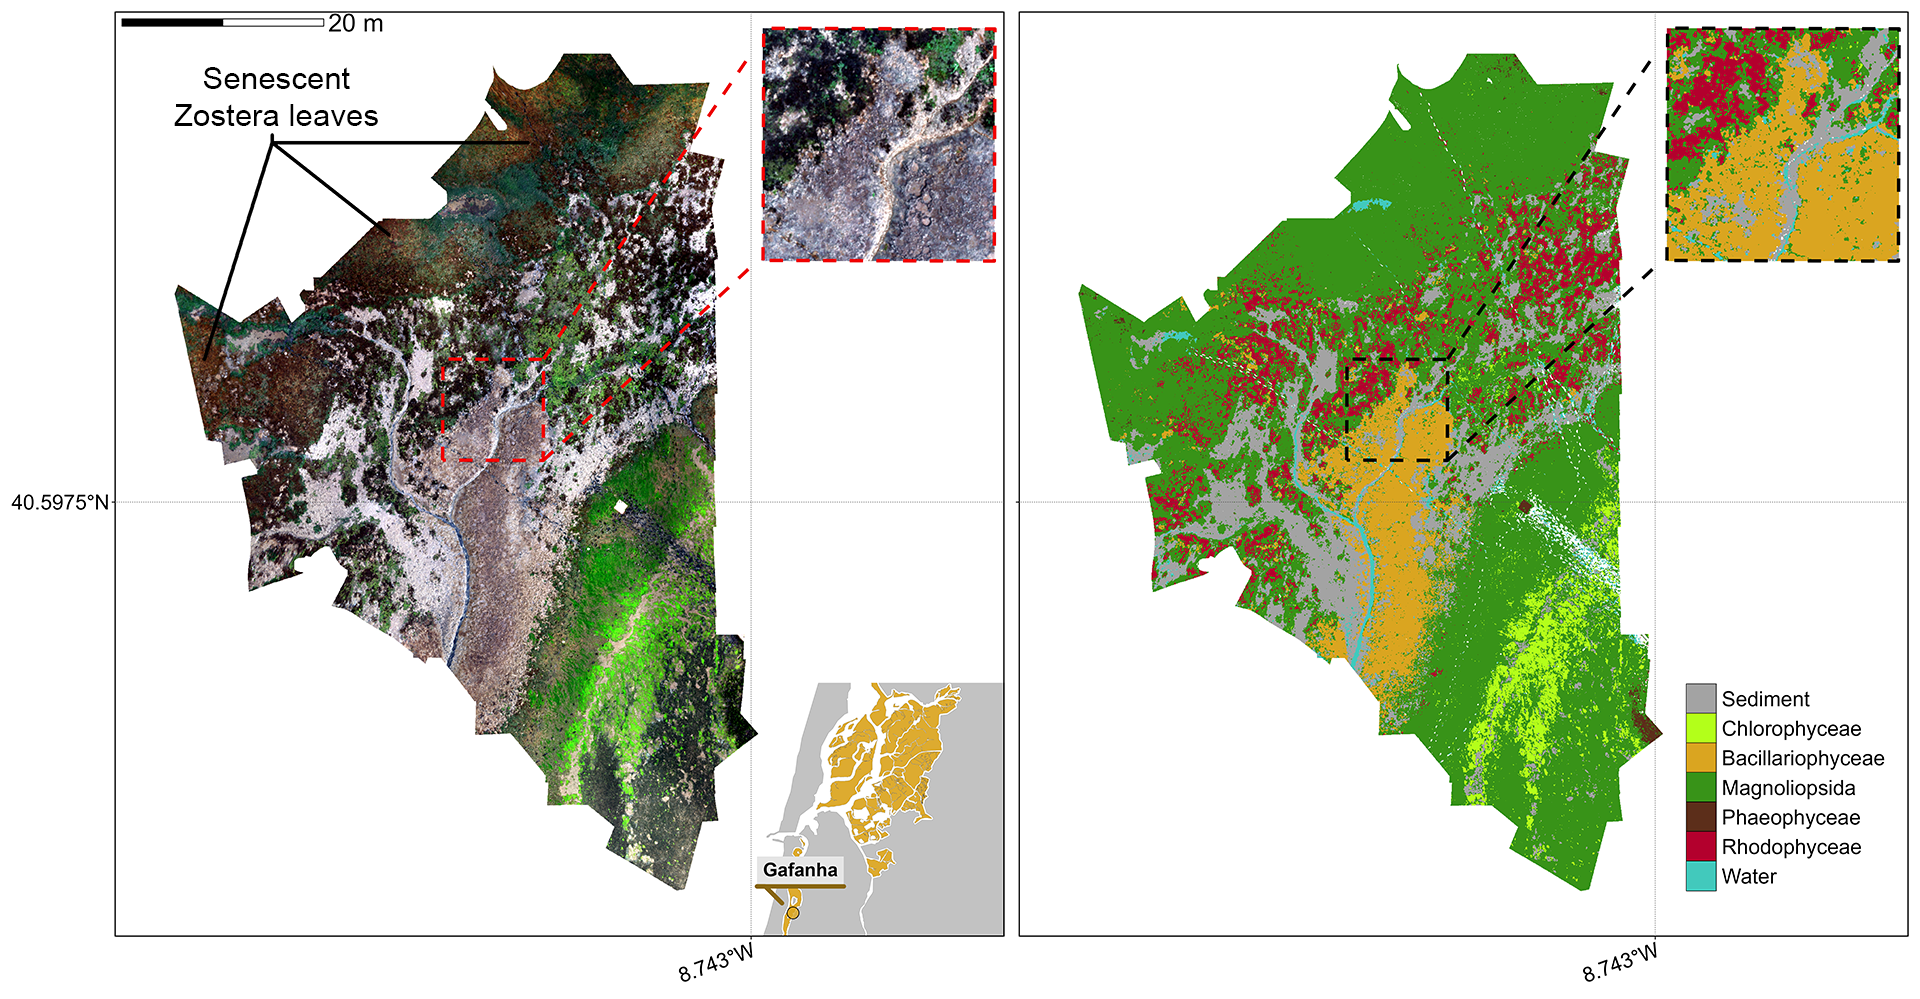
\includegraphics[width=1\linewidth,height=\textheight,keepaspectratio]{./Figures/Low_res/Maps Pred/FigX-Gaf_Low_Pred.png}

}

\caption{\label{fig-GafLow}RGB orthomosaic (Left) and Prediction (Right)
of the low altitude flight of Gafanha, Portugal. The total extent of
this flight was 3000 m² with a resolution of 8 mm per pixel. Background
colors indicate intertidal area (Light Green) and land area (Light
Grey). The zoom covers an area equivalent to a 10-meter Sentinel-2 pixel
size.}

\end{figure}%

The high-altitude flight over Gafanha covered a total area of
\textasciitilde1 km² (Figure~\ref{fig-GafHigh}). A channel contouring a
small island was masked in the prediction map. Most of vegetation area
was classified as seagrass by the model, including patches with
discolored leaves. Only a few pixels were classified as green macroalgae
(F1 score of 0.55). Patches of red macroalgae were correctly classified
(F1 score of 0.85). In the northern part of the site and near the land
eadges, patches of the schorre angiosperm \emph{Sporobolus maritimus}
(syn. \emph{Spartina maritima)} were misclassified, either as seagrass
or as brown algae (F1 score of 0.77 and 0.71, respectively).

\phantomsection\label{cell-fig-GafHigh}
\begin{figure}[H]

\centering{

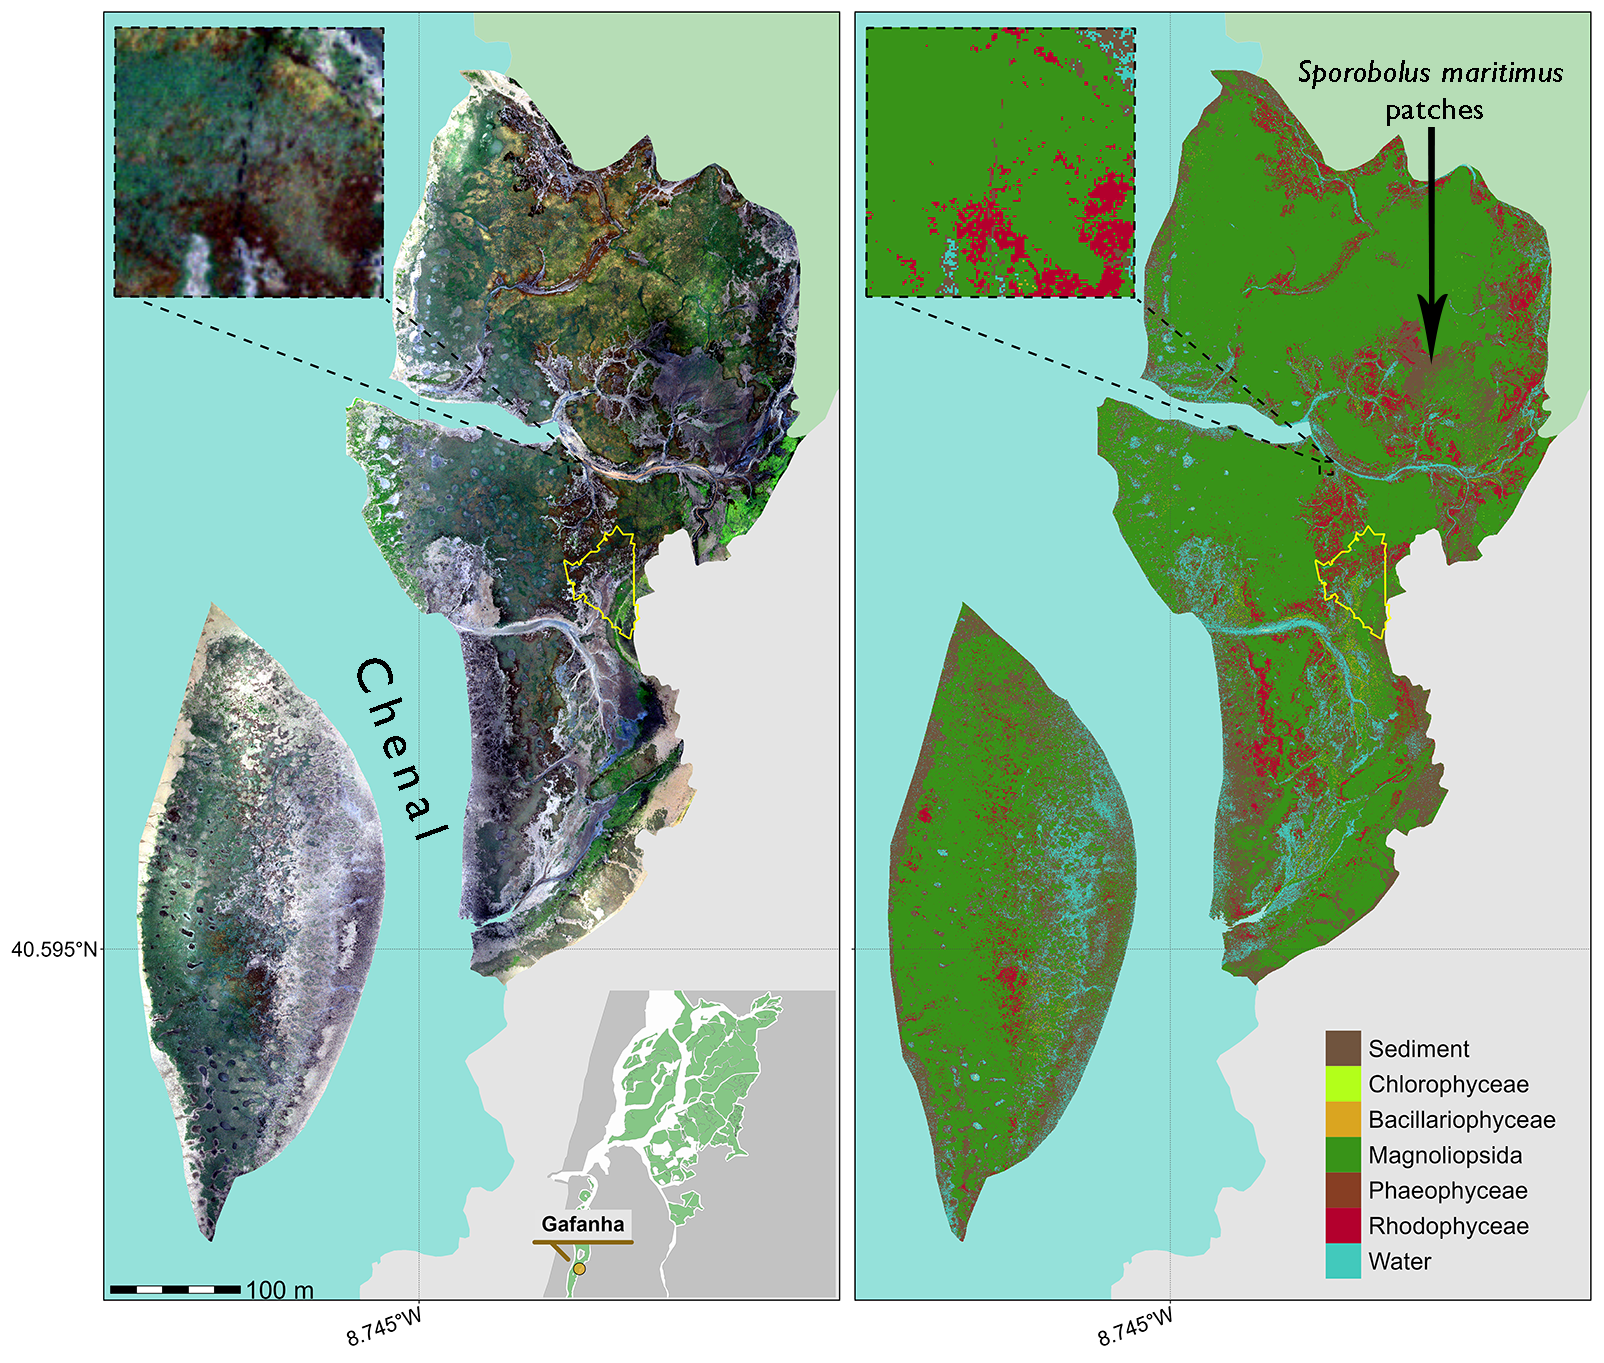
\includegraphics[width=1\linewidth,height=\textheight,keepaspectratio]{./Figures/Low_res/Maps Pred/FigX-Gaf_High_Pred1.png}

}

\caption{\label{fig-GafHigh}RGB orthomosaic (Left) and Prediction
(Right) of the high altitude flight of Gafanha, Portugal. The total
extent of this flight was about 1 km² with a resolution of 80 mm per
pixel. Background colors indicate intertidal area (Light Green), land
area (Light Grey) and water (Light Blue). The yellow outline shows the
extent of the low altitude flight of Gafanha presented in
Figure~\ref{fig-GafLow}. The zoom covers an area equivalent to a
10-meter Sentinel-2 pixel size.}

\end{figure}%

Among the high altitude flights, the one acquired over the inner part of
Ria de Aveiro coastal lagoon covered the largest area with approximately
1.5 km² (Figure~\ref{fig-Boat}). Teh vegetation present at the site was
dominated by seagrass and red macroalgae. The classification provided
consistent results, with a patchy seagrass meadow mixed with red
macroalgae on the eastern part of the site. As shown in the zoom
(Figure~\ref{fig-Boat}), the edges of the meadow were mixed with green
macroalgae (\emph{Ulva sp.}), which the model agreed with (F1 score of
0.89 for green algae, 0.97 for seagrass and 0.98 for red algae).

\phantomsection\label{cell-fig-Boat}
\begin{figure}[H]

\centering{

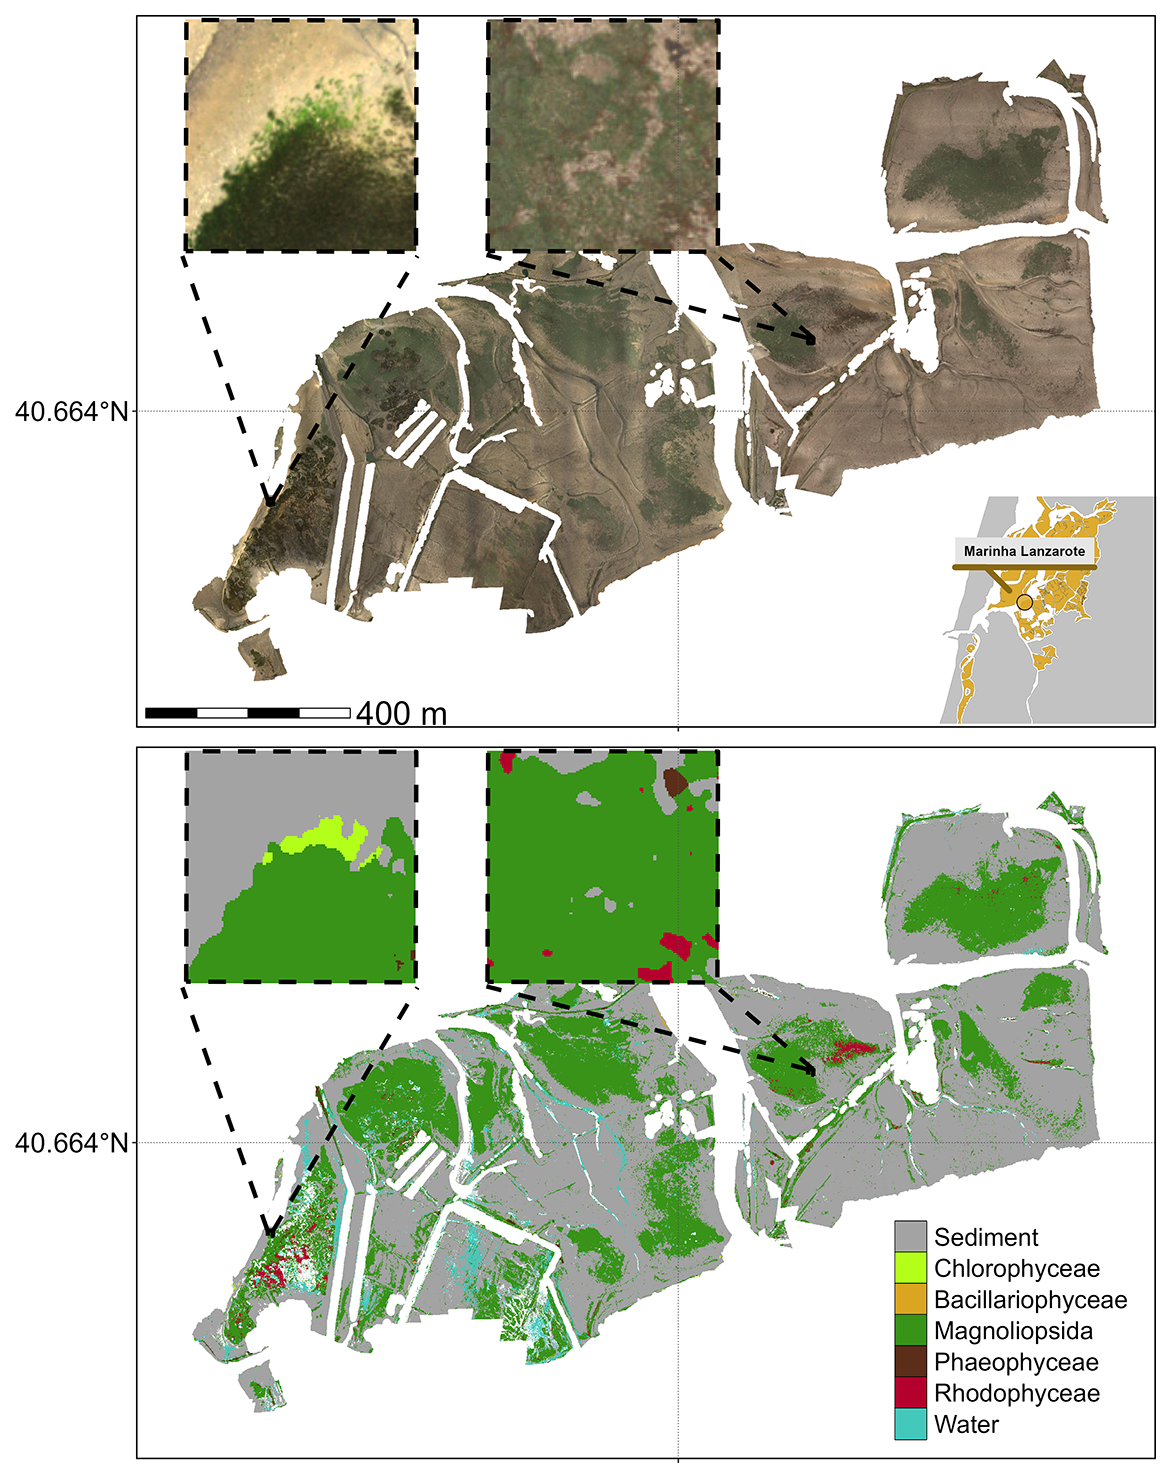
\includegraphics[width=1\linewidth,height=\textheight,keepaspectratio]{./Figures/Low_res/Maps Pred/FigX-Boat_Pred.png}

}

\caption{\label{fig-Boat}RGB orthomosaic (Top) and Prediction (Bottom)
of the flight made in the inner part of Ria de Aveiro Lagoon, Portugal.
The total extent of this flight was about 1.5 km² with a resolution of
80 mm per pixel. Background colors indicate intertidal area (Light
Green), land area (Light Grey) and water (Light Blue). The zoom inserts
cover an area equivalent to the size of a 10-meter Sentinel-2 pixel.}

\end{figure}%

The flight over L'Epine in Noirmoutier Island, France
(Figure~\ref{fig-Dike} A) was conducted near a dike, which crossed the
northern part of the site from West to East. Alongside this dike, Fucale
brown macroalgae (\emph{Fucus spp.}, \emph{Ascophyllum nodosum}) were
attached to sparse rocks, and stranded green algae (\emph{Ulva spp.})
could be observed, which was correctly reproduced by the prediction
(Figure~\ref{fig-Dike} B). This site was characterized by a high mixture
between green macroalgae and seagrass but these two classes were
correctly discriminated by the classifier (F1 score of 0.97 and 0.98
respectively).

\phantomsection\label{cell-fig-Dike}
\begin{figure}[H]

\centering{

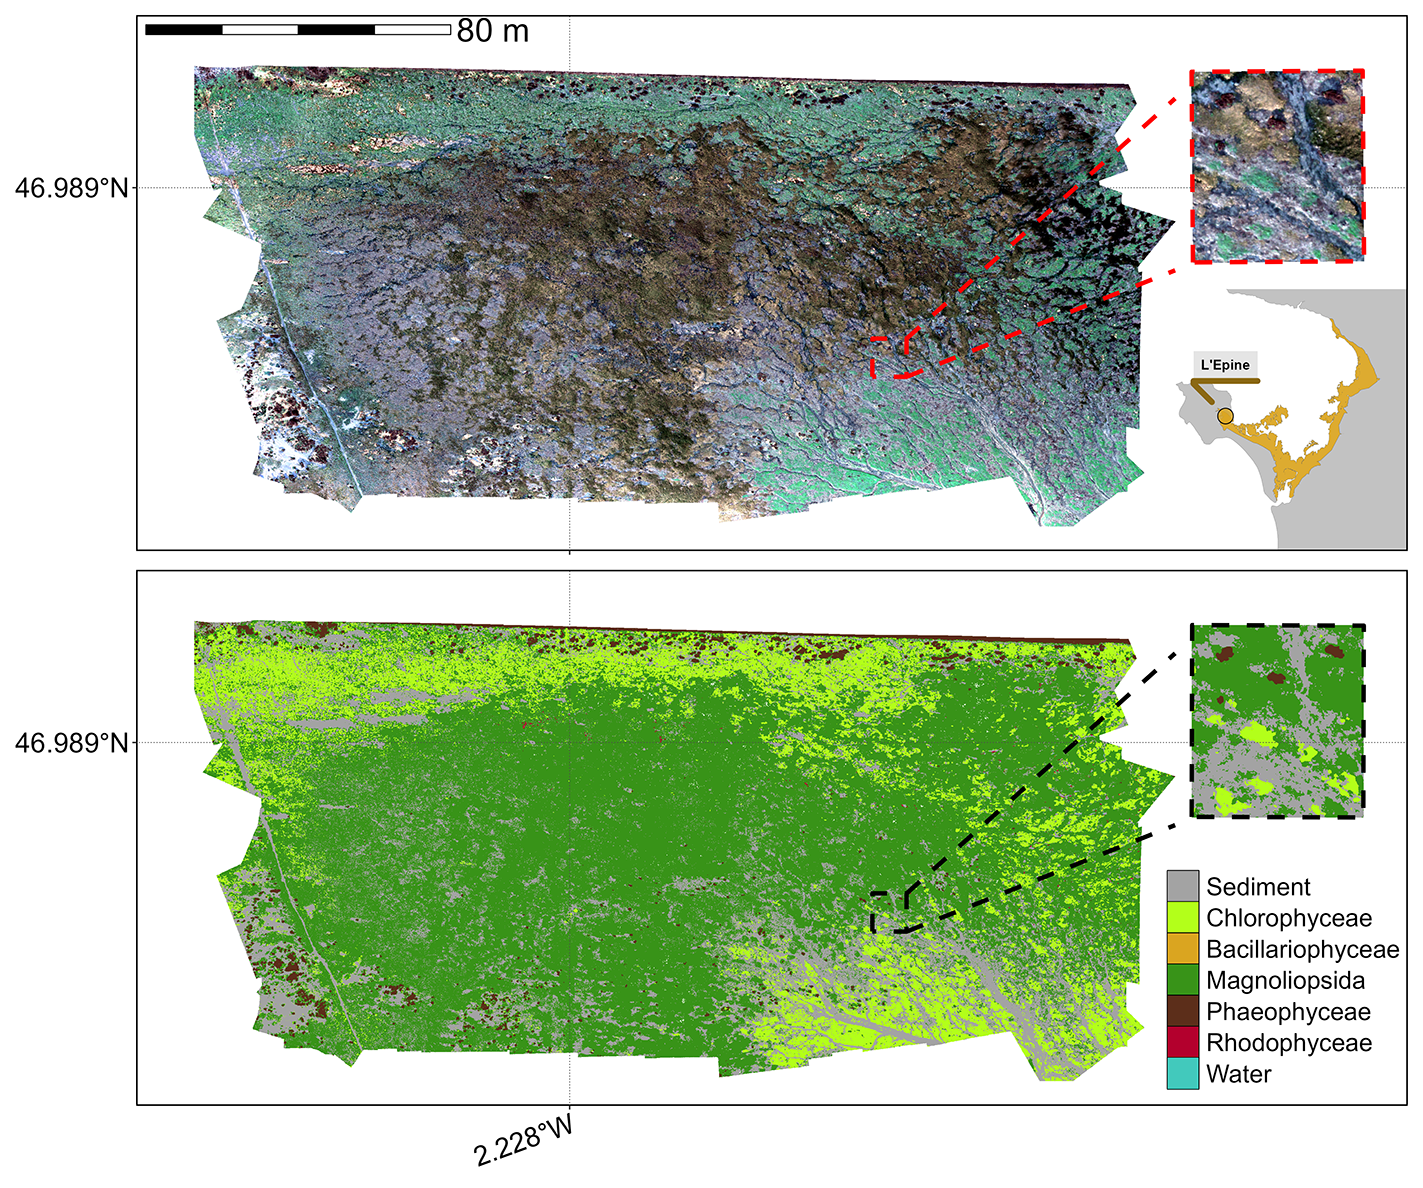
\includegraphics[width=1\linewidth,height=\textheight,keepaspectratio]{./Figures/Low_res/Maps Pred/FigX-Dike_Pred.png}

}

\caption{\label{fig-Dike}RGB orthomosaic (Top) and Prediction (Bottom)
of L'Epine, France. The total extent of this flight was about 28 000 m²
with a resolution of 80 mm per pixel. Background colors indicate
intertidal area (Light Green) and land area (Light Grey). The zoom
covers an area equivalent to a 10-meter Sentinel-2 pixel size.}

\end{figure}%

\subsection{Validation of the model}\label{validation-of-the-model}

With all drone flights combined, the model global accuracy was 94.26\%
with a Kappa coefficient of 0.92 (Figure~\ref{fig-Validation}).

\phantomsection\label{cell-fig-Validation}
\begin{figure}[H]

\centering{

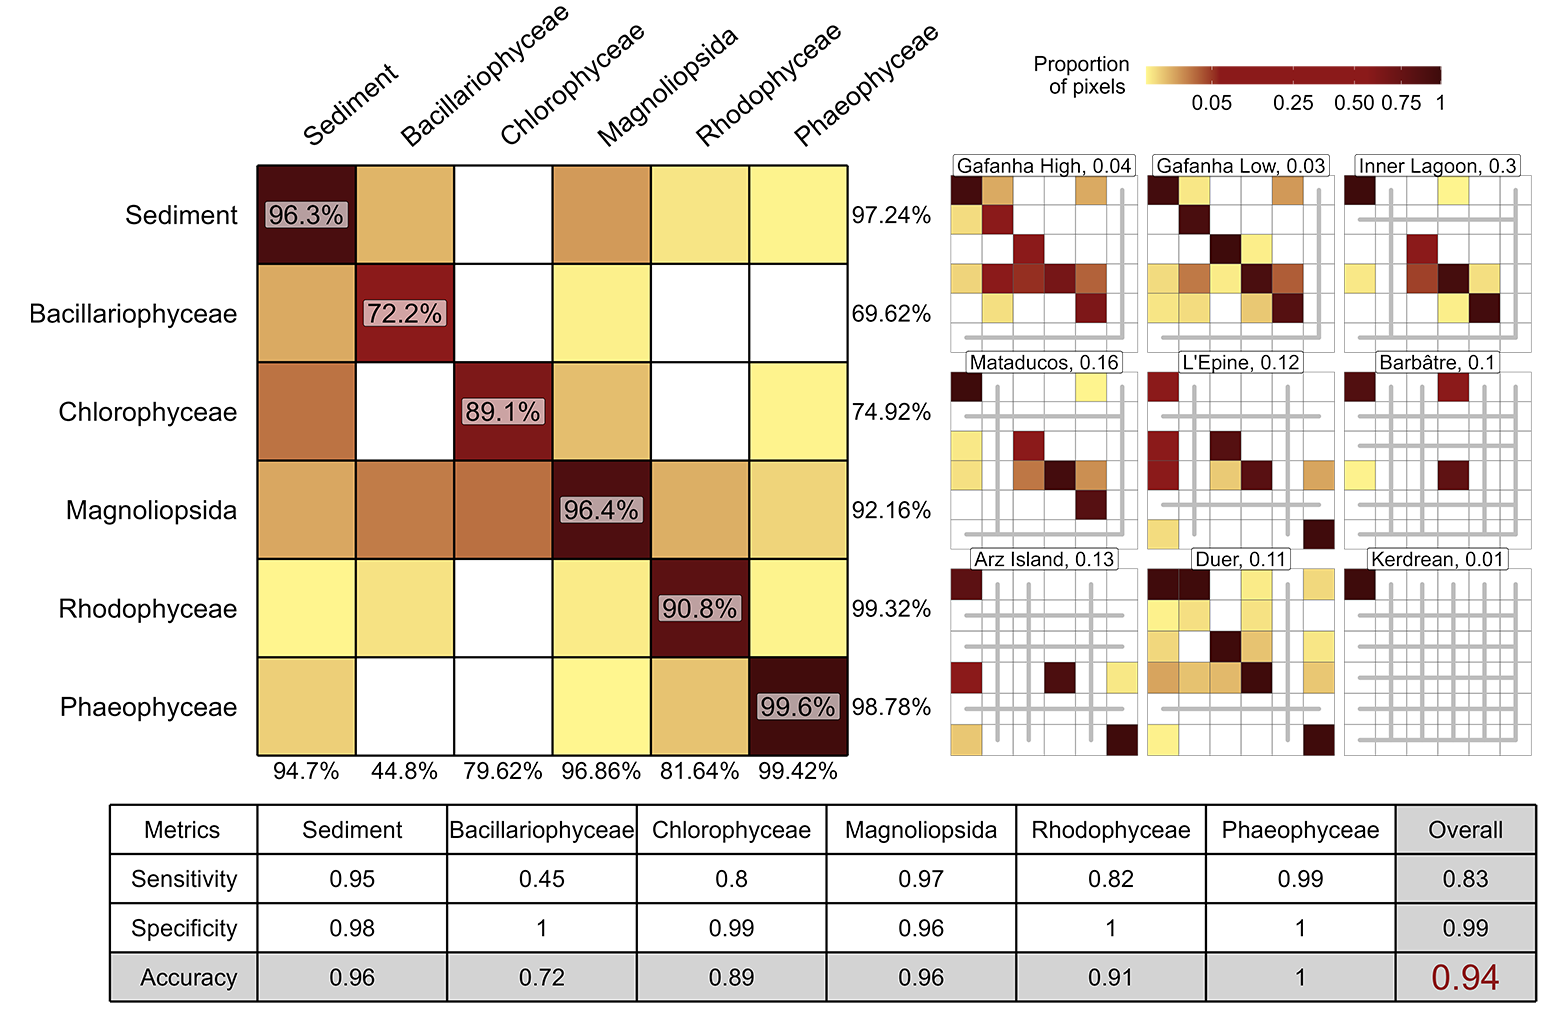
\includegraphics[width=1\linewidth,height=\textheight,keepaspectratio]{./Figures/Low_res/Validation/ConfusionMatrixGlobal.png}

}

\caption{\label{fig-Validation}A global confusion matrix on the left is
derived from validation data across each flight, while a mosaic of
confusion matrices from individual flights is presented on the right.
The labels inside the matrices indicate the balanced accuracy for each
class. The labels at the bottom of the global matrix indicate the User's
accuracy for each class, and those on the right indicate the Producer's
Accuracy. The values adjacent to the names of each site represent the
proportion of total pixels from that site contributing to the overall
matrix. Grey lines within the mosaic indicate the absence of validation
data for the class at that site. The table at the bottom summarizes the
Sensitivity, Specificity, and Accuracy for each class and for the
overall model.}

\end{figure}%

The lowest performing site was Gafanha High (global accuracy of 75.45\%)
whereas Mataducos was the site with the most accurate prediction (global
accuracy of 98.05\%). Overall, the classes Phaeophyceae, Magnoliopsida,
Sediment and Rhodophyceae were correctly classified with a balanced
accuracy of 1, 0.96, 0.96 and 0.91 respectively. Bacillariophyceae was
the least accurate class (accuracy of 0.72 ) mainly due to confusion
with Magnoliopsida and Sediment.

\subsection{Variable importance}\label{variable-importance-1}

The computation of the variable importance made it possible to identify
which bands were the most useful for class prediction
(Figure~\ref{fig-VIP}).

\phantomsection\label{cell-fig-VIP}
\begin{figure}[H]

\centering{

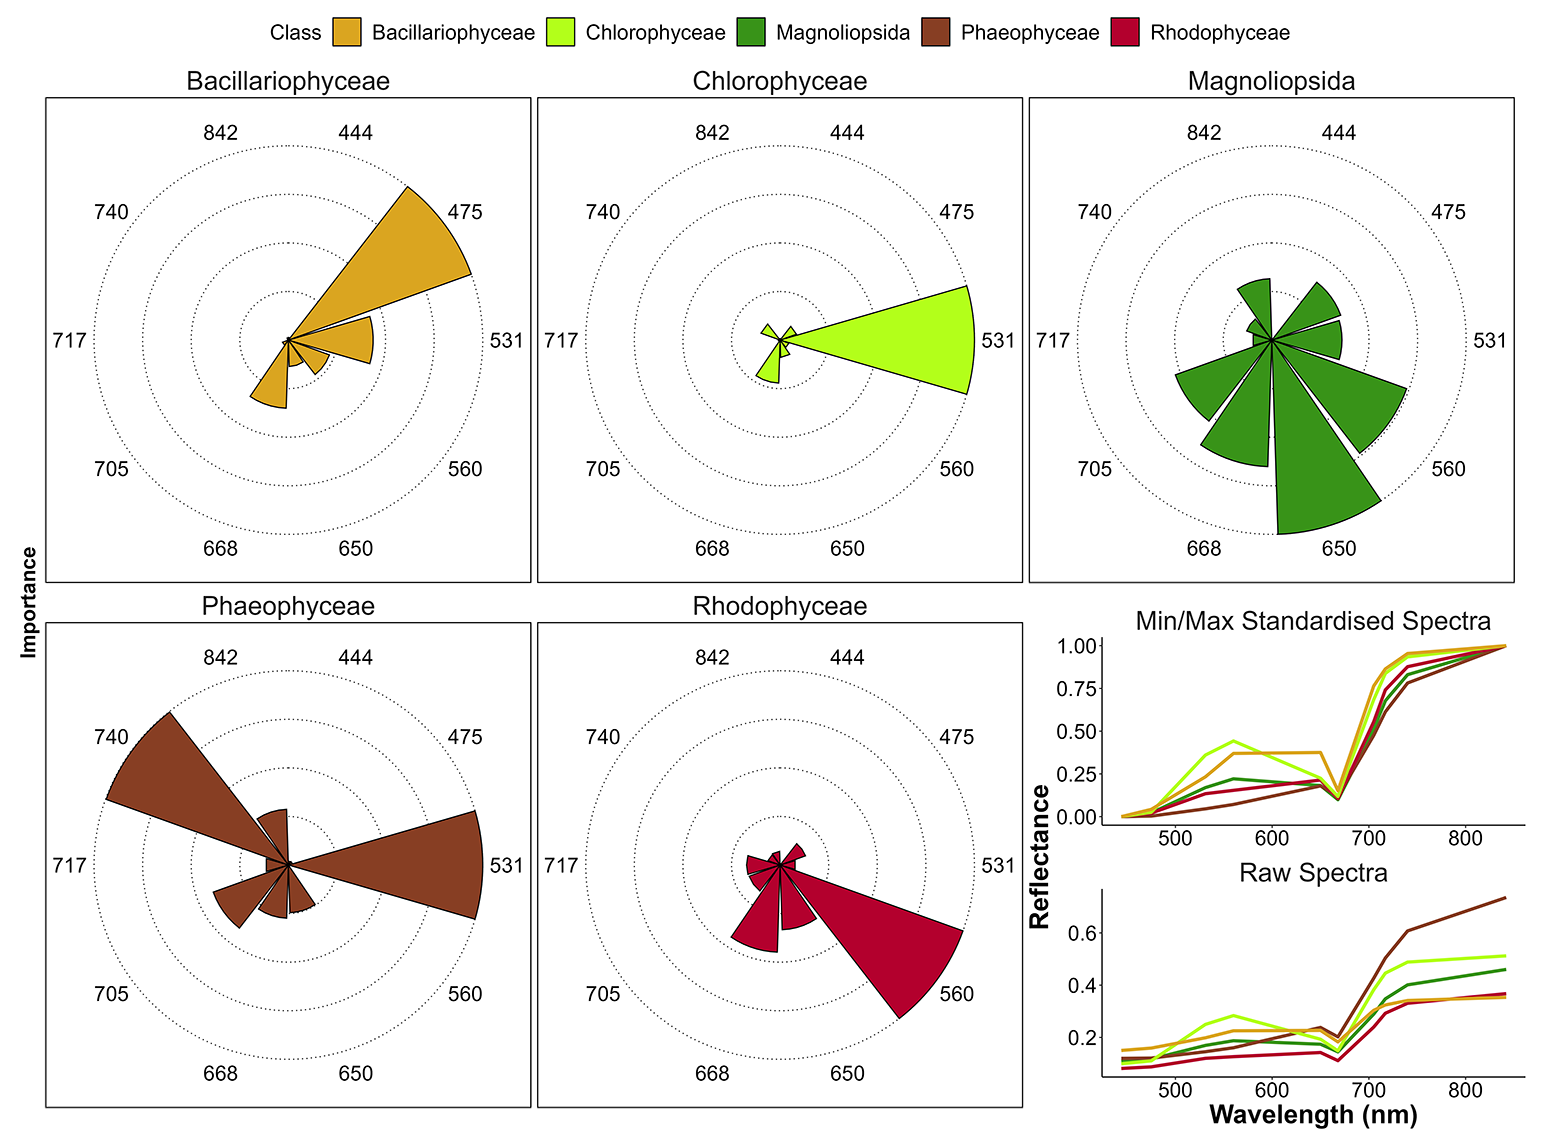
\includegraphics[width=1\linewidth,height=\textheight,keepaspectratio]{Figures/Low_res/VIP/Fig_VIP.png}

}

\caption{\label{fig-VIP}Variable Importance of the Neural Network
Classifier for each taxonomic class. The longer the slice, the more
important the variable for prediction of each class. The right plot
shows the drone raw and standardised reflectance spectra of each class.
Each slice represents the Variable Importance (VI) of both raw and
standardised reflectance combined.}

\end{figure}%

The spectral bands at 444, 717 and 842 nm of the Micasense camera did
not provide important information to discriminate any of the vegetation
classes. The band at 531 nm was the most important predictor by far for
the classifier to accurately predict Chlorophyceae. In fact, at this
wavelength, the Chlorophyceae spectra showed the highest reflectance
among all vegetation classes (Figure~\ref{fig-vegetation} F). The bands
at 531 and 740 nm were the most important predictors for Phaeophyceae,
corresponding to the lowest reflectance among all classes. Bands at 475
and 560 nm were the most important predictors for Bacillariophyceae and
Rhodophyceae, respectively. Four predictors, ranging from the green (560
nm) to the RedEdge (705 nm) bands were important to accurately predict
Magnoliopsida.

\subsection{Effect of spatial resolution on the
classification}\label{effect-of-spatial-resolution-on-the-classification}

Clear differences were seen in vegetation loss across different
resolutions and vegetation classes (Figure~\ref{fig-pixelsize}). At a
fine resolution of 1m, changes in the retrieved area for each vegetation
type are minimal. Green algae shows the highest loss, with 1.2\% area
lost compared to the native resolution (80 mm). As the resolution
coarsens to 10m, vegetation loss becomes more pronounced, with green
macroalgae again experiencing the greatest reduction (12\% compared to
8cm) and seagrass showing the smallest loss (1.3\%). At a resolution of
30m, all green algae have been lost (100\% compared to 8cm), while
seagrass experiences a relatively small reduction of 11\%. Brown
macroalgae and red macroalgae show moderate declines, with losses at 30m
resolution reaching approximately 37\% and 59\%, respectively.

\phantomsection\label{cell-fig-pixelsize}
\begin{figure}[H]

\centering{

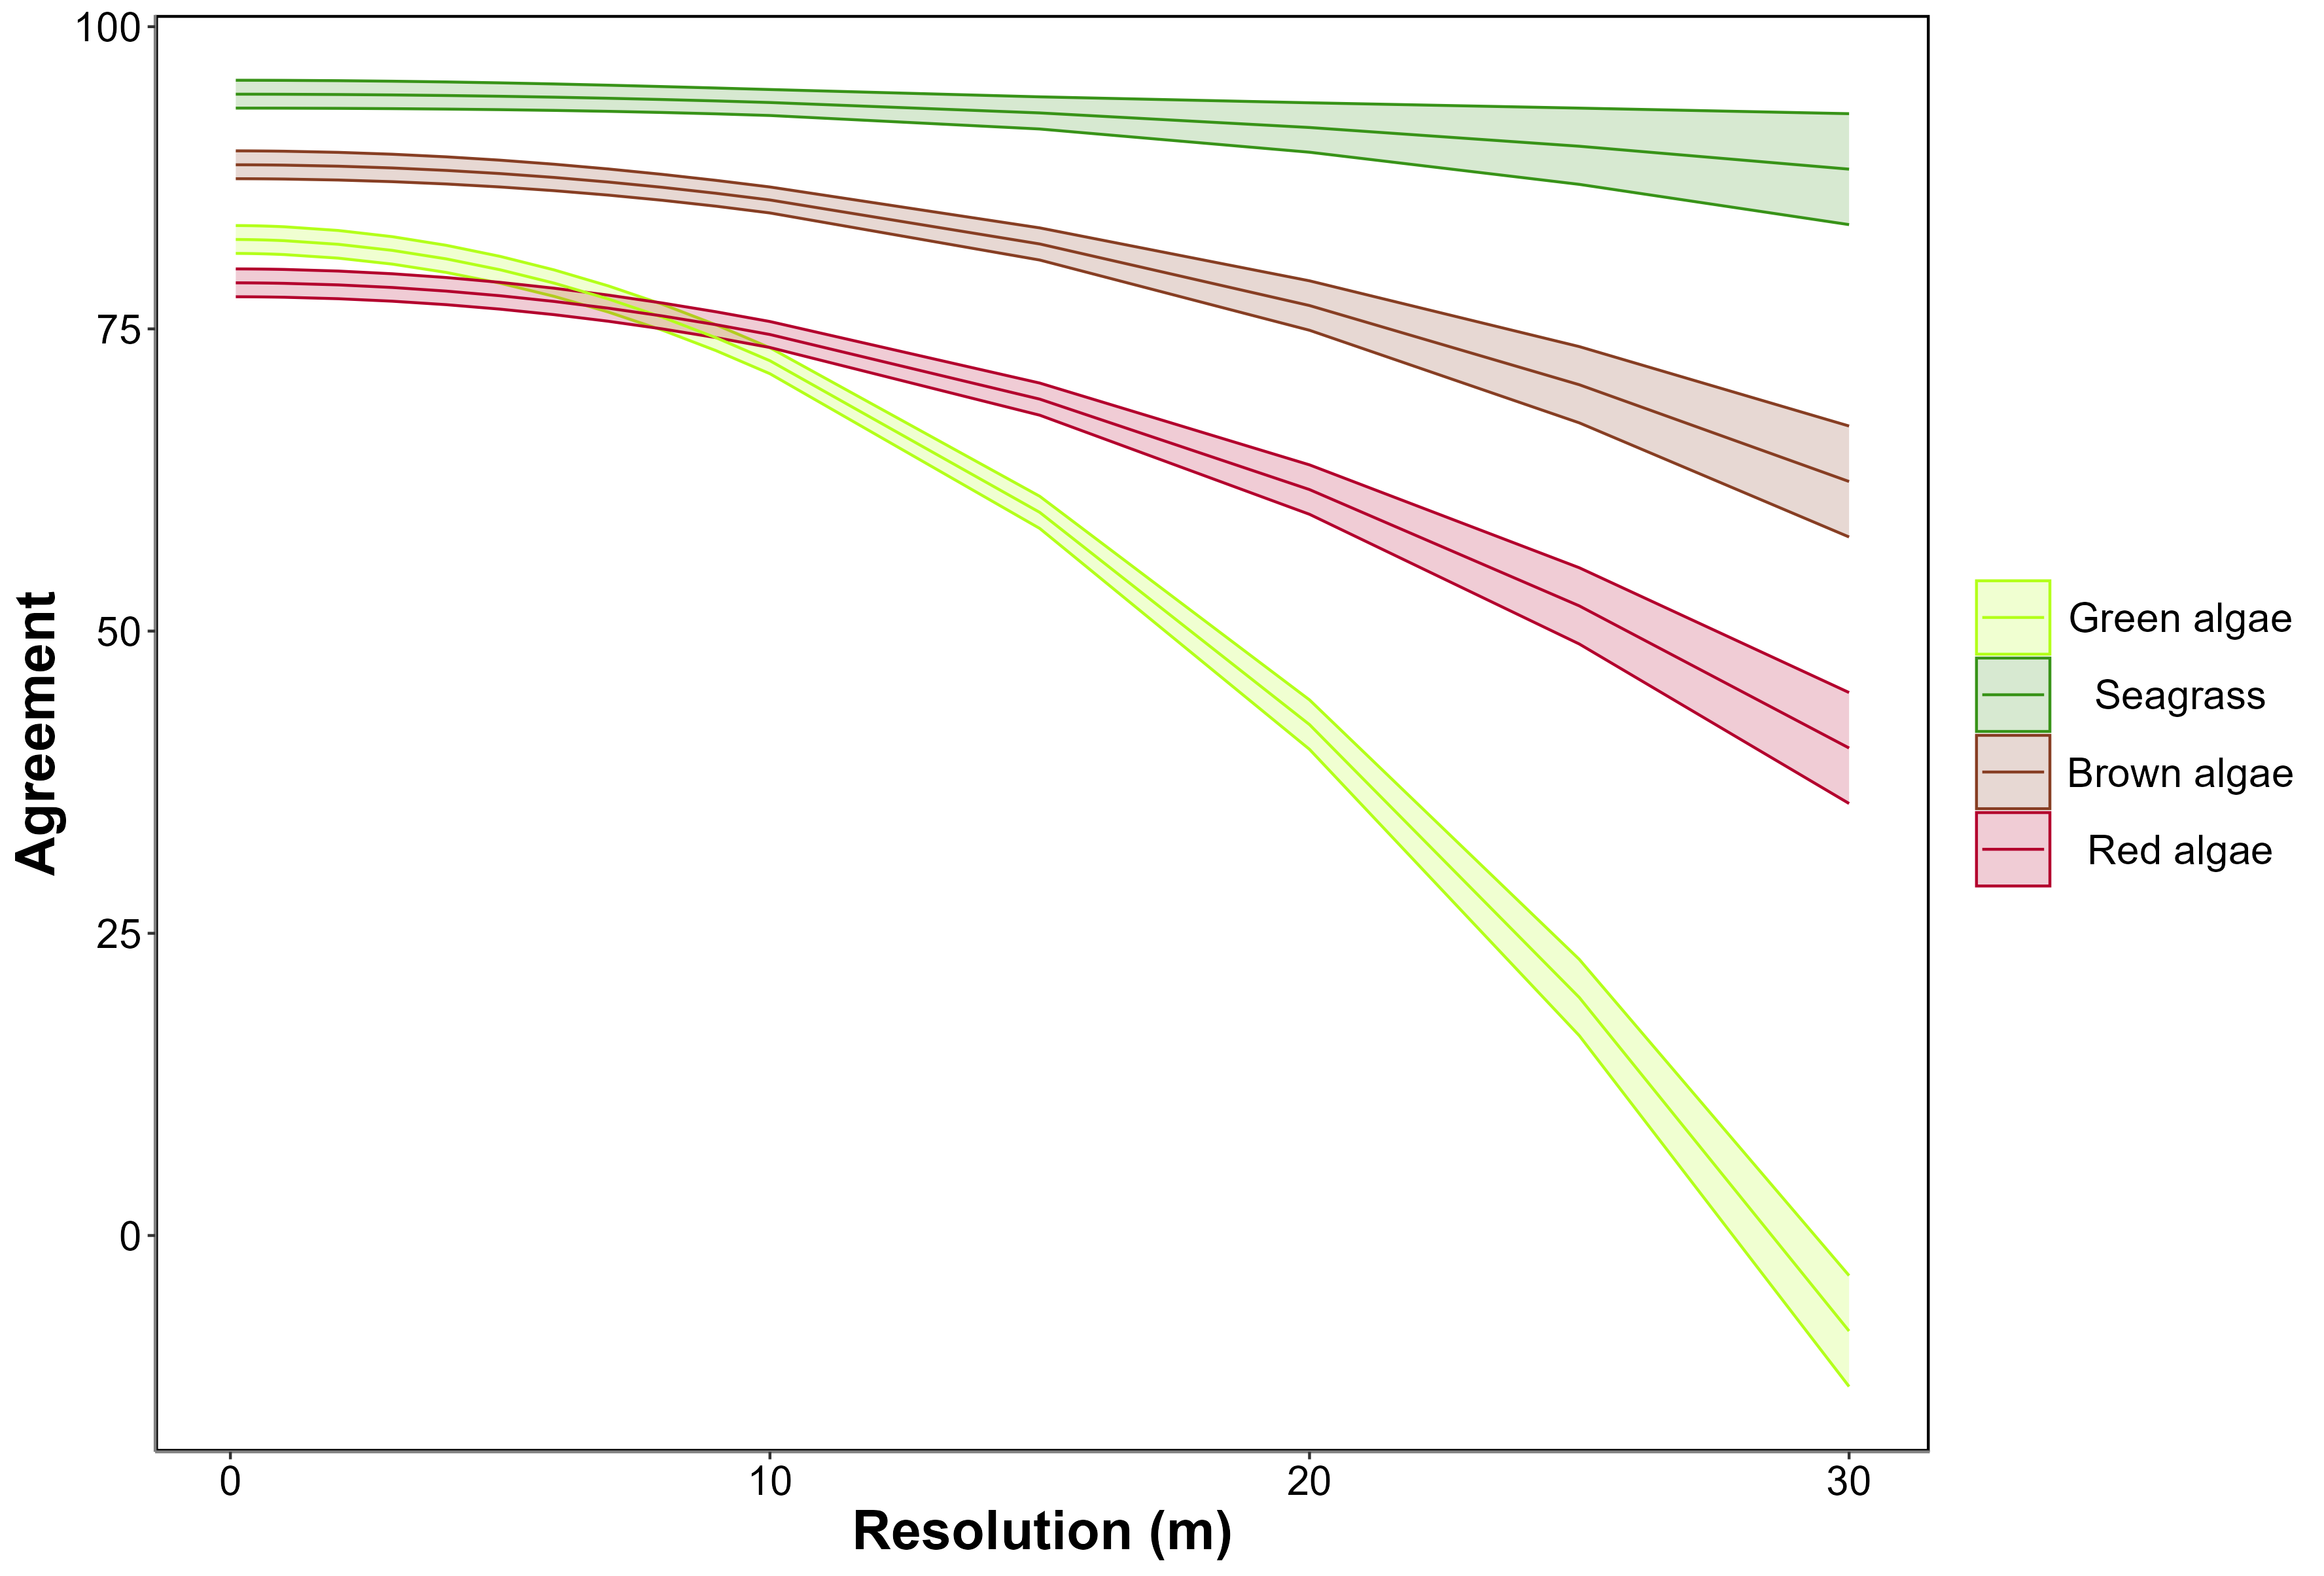
\includegraphics[width=0.9\linewidth,height=\textheight,keepaspectratio]{Figures/High_res/resolution_plot.png}

}

\caption{\label{fig-pixelsize}Predicted area loss for different
vegetation types (green algae, seagrass, brown algae, red algae) as a
function of spatial resolution. Lines represent Generalized Linear Model
(GLM) predictions, and shaded areas indicate standard errors. As
resolution decreases, predicted area loss increases for all vegetation
types, with green algae showing the highest loss and seagrass the
smallest at coarser resolutions.}

\end{figure}%

\subsection{Effect of the percent cover on the
prediction}\label{effect-of-the-percent-cover-on-the-prediction}

Using the very high resolution low altitude flight (8 mm pixels), we
determined the minimal percent cover required to correctly classify a
given class within the corresponding high altitude flight (8cm pixel
resolution ; Figure~\ref{fig-upscaling}).

\phantomsection\label{cell-fig-upscaling}
\begin{figure}[H]

\centering{

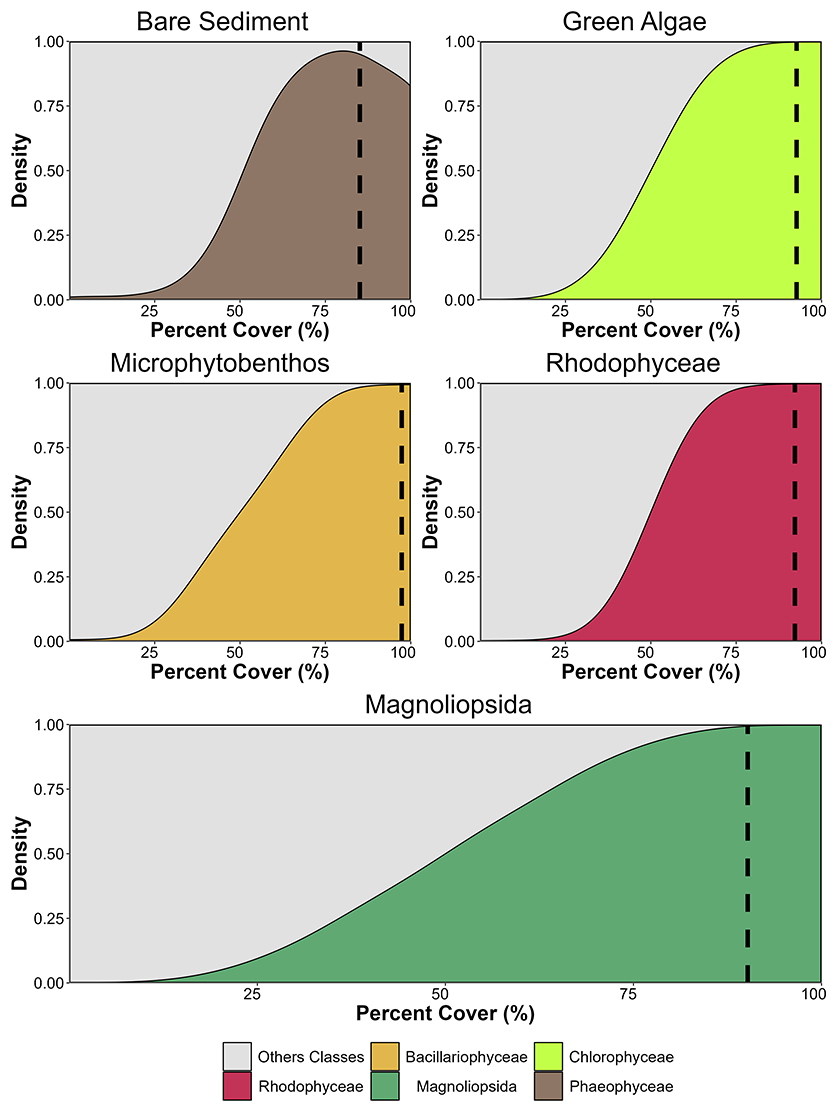
\includegraphics[width=0.9\linewidth,height=\textheight,keepaspectratio]{Figures/Low_res/Upscaling/density_vs_Proportion.png}

}

\caption{\label{fig-upscaling}Kernel density plot showing the proportion
of pixel well classified based on the percent cover of the class in high
altitude flight pixels of Gafanha, Portugal. Each subplot shows all the
pixels of the same classes on the high altitude flight. Percent cover of
classes was retrieved using the result of the classification of the low
altitude flight of Gafanha, Portugal.}

\end{figure}%

A percent cover of at least 80\% was sufficient to have all the 80 mm
pixels correctly classified, with the exception of Magnoliopsida that
required a higher cover (\textgreater90 \%) to be accurately classified.
Concerning the probability of each class, there is a linear relationship
between the percent cover and the confidence of the model to predict the
class. To predict green macroalgae with a model likelihood of 0.85, a
cover of 93 \% was needed, 90 \% for seagrass, 92 \% for red macroalgae
and 97 \% for diatoms When the vegetation cover of a given class was 100
\%, coarser high-flight pixels were correctly classified for all the
classes except for Bare Sediment, which was only correctly classified
80\% of the time. This phenomenon may be attributed to the time gap
between the two flights, allowing for microphytobenthos migration to the
sediment surface during low tide, consequently altering the model's
classification from bare sediment to Bacillariophyceae.

\section{Discussion}\label{discussion}

\subsection{Vegetation Discrimination}\label{vegetation-discrimination}

The primary objective of this study was to develop a method for the
accurate classification of emerged macrophytes observed during low tide
on tidal flats, specifically focusing on distinguishing between
Chlorophyceae (green macroalgae) and marine Magnoliopsida (seagrasses)
using a multispectral resolution. The discrimination between seagrasses
and green macroalgae is challenging due to their optical similarity in
the visible range
\citep{oiry2021using, bannari2022, veettil2020opportunities}. These two
macrophytes share a similar pigment composition: chlorophyll-a (common
to all vegetation types), chlorophyll-b (an additional photosynthetic
pigment), and accessory carotenoids such as zeaxanthin, lutein and
neoxanthin (Figure~\ref{fig-Pigm}). Their spectral responses could be
close, particularly at a multispectral resolution. Seagrass and green
macroalgae frequently co-occur in intertidal areas, and can intermingle
within a remote sensing pixel if the spatial resolution is too low.
Here, the issue of intra-pixel mixing was resolved thanks to the very
high spatial resolution of the drone (from 8 to 80 mm). In this study
the risk of spectral confusion was avoided with a machine-learning
approach exploiting a neural networks classifier. Our drone flights and
a recent study based on \emph{in situ} radiometry, suggested that a
sensor with at least eight spectral bands ranging from 500 to 850 nm,
and including a green band at 530 nm and a RedEdge band at 730 nm, was
crucial to accurately discriminate green macroalgae from seagrasses
\citep{Davies2023}.

\phantomsection\label{cell-fig-Pigm}
\begin{figure}[H]

\centering{

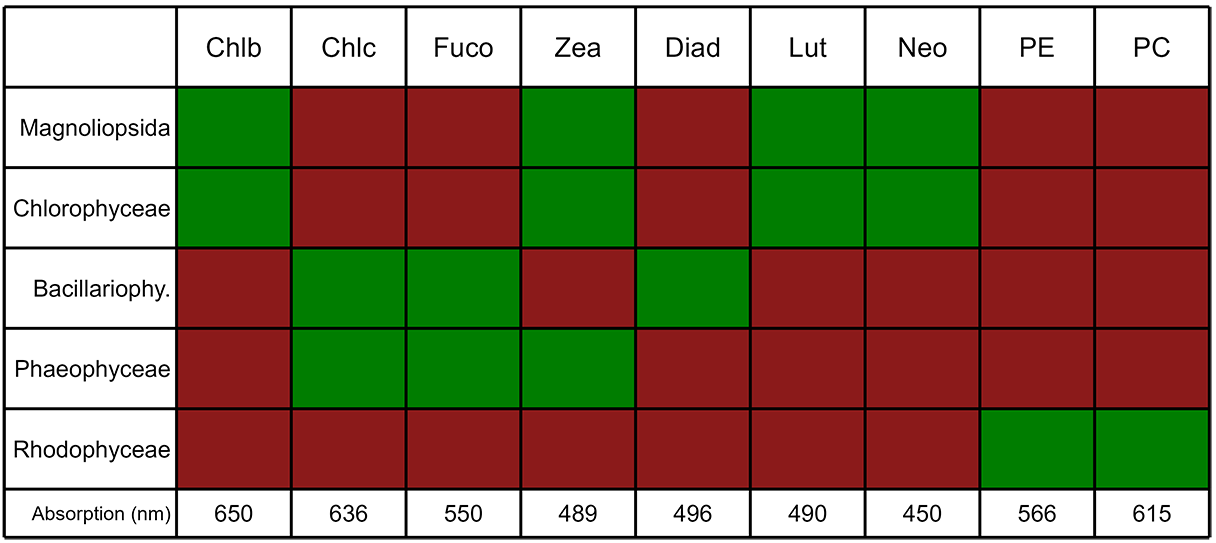
\includegraphics[width=1\linewidth,height=\textheight,keepaspectratio]{./Figures/Low_res/Disc_Pigment_Table.png}

}

\caption{\label{fig-Pigm}Photosynthetic and carotenoid pigments present
(Green) or absent (Red) in each taxonomic class present in the Neural
Network Classifier, along with their absorption wavelength measured with
spectroradiometer, Chl-b: chlorophyll-b, Chl-c: chlorophyll-c, Fuco:
fucoxanthin, Zea: zeaxanthin, Diad: diadinoxanthin, Lut: lutein, Neo:
neoxanthin, PE: phycoerythrin, PC: phycocyanin
\citetext{\citealp{ralph2002}; \citealp[
\citep{christensen1977seaweeds}]{Douay2022}; \citealp{cartaxana2016regulation}; \citealp{meleder2013vivo}}.}

\end{figure}%

\phantomsection\label{cell-fig-ValidationGreen}
\begin{figure}[H]

\centering{

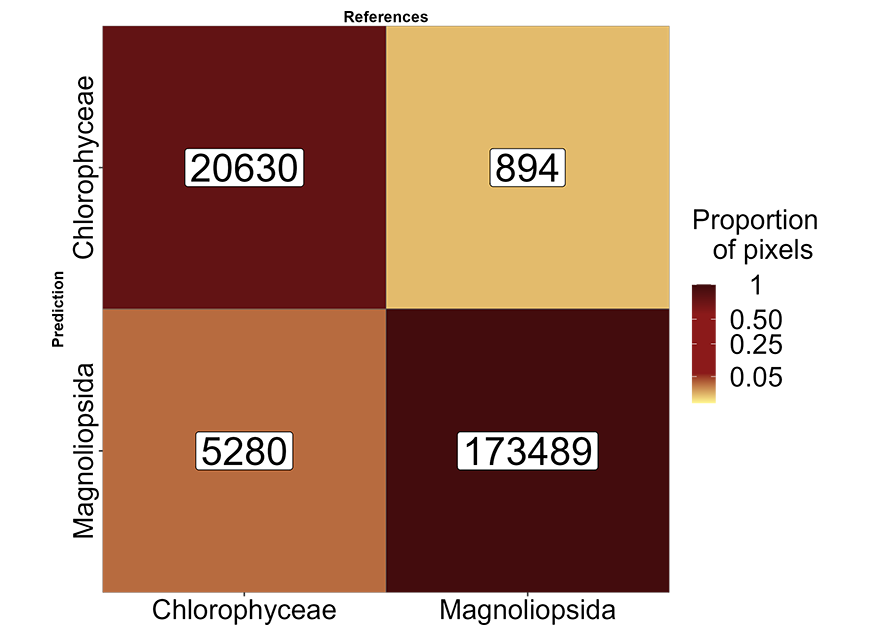
\includegraphics[width=1\linewidth,height=\textheight,keepaspectratio]{./Figures/Low_res/Validation/ConfusionMatrixGreen.png}

}

\caption{\label{fig-ValidationGreen}Sample of
Figure~\ref{fig-Validation} focusing on green macrophytes. The labels
inside the matrix indicate the number of pixels.}

\end{figure}%

Meeting these two criteria, the Micasense RedEdge-MX DUAL camera used in
this study, enabled the classifier to achieve 97\% of accuracy between
these two classes (Figure~\ref{fig-ValidationGreen}). Even if their
pigment composition is similar, differences in the spectral shape can be
observed, with green algae having a higher reflectance peak at 560 nm as
well as a higher NIR plateau than seagrass
(Figure~\ref{fig-vegetation}). Such differences were previously
attributed to differences in pigments concentration and/or ratios
\citep{bargain2013seasonal}, cellular structure as well as in the
orientation of the plant at the sediment surface
\citep{beach1997vivo, kirk1994light, hedley2018influence}.

The variable importance analysis (Figure~\ref{fig-VIP}) identified that
the band at 531 nm was the most important for accurately identifying
Chlorophyceae. In fact, at this wavelength, Chlorophyceae exhibited the
highest reflectance among all other classes, highlighting the difference
in carotenoid to chlorophyll-a ratios between seagrasses and green
macroalgae \citep{repolho2017seagrass}. Concerning Phaeophyceae, the
thick cell walls of these macroalgae \citep{charrier2021growth} make it
more reflective in the infrared part of the spectra \citep{Slaton2001},
while the presence of fucoxanthin and zeaxanthin result in a low
reflectance in the visible region (Figure~\ref{fig-VIP} ;
Figure~\ref{fig-Pigm}). These two key features have been identified by
the Neural Network as the two principal predictors to accurately
identify brown algae (Figure~\ref{fig-VIP}). Similarly, the presence of
phycoerythrin and phycocyanin in Rhodophyceae contribute to the lowest
reflectance among all classes in the spectral range from 560 to 615 nm
(Figure~\ref{fig-VIP}). Indeed the band at 560 nm has been identified as
important for identifying this class, likely due to phycoerythrin
absorption at this wavelength. Regarding Bacillariophyceae, 475 nm was
the most important predictor for this class (Figure~\ref{fig-VIP}).
Indeed, the reflectance at 475 nm was higher for Bacillariophyceae than
for any other vegetation class (Figure~\ref{fig-vegetation}), very
likely due to the low biomass (and associated concentration of
blue-absorbing pigments) of these unicellular organisms compared to
seagrass and macroalgae.

\subsection{Altitude and Temporal Effects on Vegetation Prediction
Accuracy}\label{altitude-and-temporal-effects-on-vegetation-prediction-accuracy}

The ability to differentiate between various types of vegetation plays a
critical role in ecological monitoring and coastal management
\citep{WFD2000}. By distinguishing between seagrasses and macroalgae,
our approach facilitates targeted conservation strategies, enabling more
effective preservation and restoration efforts in coastal ecosystems.
While comparing the reflectance at two different altitudes (12 m and 120
m with a spatial resolution of 8 and 80 mm, respectively), a nearly
one-to-one relationship was observed, with a Root Mean Square Error
(RMSE) of 0.02 (Figure~\ref{fig-CompareRef}). This result indicates that
the reflectance measured by remote sensing (RS) sensors is not
significantly influenced by pixel size. This finding is valuable for
integrating drone-based data into larger-scale mapping projects (e.g.,
combining satellite and drone mapping in side-by-side analyses). The
consistency of reflectance across altitudes suggests that drones can be
effectively used for finer-scale mapping without compromising data
accuracy when merging with other platforms. However, it was observed
that there is an underestimation of the infrared part of the spectra in
the high-altitude dataset (Figure~\ref{fig-CompareRef}). Such disparity
in infrared reflectance may stem from temporal differences between the
flights, possibly resulting in a slightly drier intertidal area and
consequently higher infrared reflectance. This disparity poses an issue
for the methodology followed in the present study, relying solely on one
flight height for training. To address this issue, we employed min/max
standardized reflectance spectra as predictors for the model
Equation~\ref{eq-std}. This approach allowed us to eliminate the slight
reflectance difference between the flights (Figure~\ref{fig-CompareRef}
B) and to focus on the shape of the spectra in the visible part of the
electromagnetic spectra, where different pigmentation are associated to
taxonomic diagnostic features. In contrast to subtidal seagrasses, which
maintain a relatively constant biomass throughout the year, intertidal
seagrasses, like the one studied in this work, exhibit strong seasonal
phenology \citep{davies2024sentinel}. At some sites, they completely
disappear during the winter and reach their peak above-ground biomass in
the summer and early autumn. Along with these seasonal changes in
biomass, the pigment composition and ratios also vary throughout the
year, reflecting the plants' adaptations to different environmental
conditions \citep{bargain2013seasonal, legare2022remote}.
Standardization of spectral signatures helps to mitigate the impact of
changing biomass on the spectral profile, enabling the development of a
model that can reliably predict vegetation across different geographical
locations and seasons. This approach allows for consistent
classification of vegetation despite variations in biomass and
fluctuations in light conditions, providing a robust tool for monitoring
and predicting vegetation dynamics
\citep{fyfe2003spatial, COSTA2021107018, piaser2023impact}. We found 90
\% seagrass cover was necessary at an 8 cm resolution for confident
prediction of its presence (Figure~\ref{fig-upscaling}). However, due to
the strong phenology of intertidal seagrass meadows in Europe, the
period when a meadow is well-established can be temporally restricted,
limiting the ideal window for accurate detection.

\subsection{Impact of Pixel Resolution on the prediction and
Implications for Satellite Remote
Sensing}\label{impact-of-pixel-resolution-on-the-prediction-and-implications-for-satellite-remote-sensing}

Pixel resolution plays a critical role in accuratly retrieving
vegetation area from remote sensing data. As pixel size increases, we
found a consistent decline in area retrieval is observed across all
vegetation types, with more pronounced effects for certain types, such
as green algae (Figure~\ref{fig-pixelsize}). This highlights the
sensitivity of spatial resolution in detecting smaller or more
fragmented vegetation features. Green algae, being particularly patchy
across all study sites, shows the steepest decline in areal agreement as
pixel size increases, which aligns with expectations given the
limitations of coarser resolution in capturing fine-scale details.

This resolution-area relationship has important implications for
satellite missions like Sentinel-2 and Landsat, which are commonly used
in marine and coastal vegetation studies. Both satellites offer
high-resolution imagery, with pixel sizes of 10m and 30m, respectively.
While these resolutions are suitable for broad-scale environmental
monitoring, they may be too coarse to capture finer-scale heterogeneity,
particularly in fragmented vegetation like green algae. Our findings
suggest that, while the 30m resolution of Landsat may be adequate for
homogeneous vegetation types, such as seagrass, a higher resolution is
essential for accurately mapping patchy vegetation like green algae.
These findings have direct implications for environmental management and
conservation planning. Overlooking fine-scale vegetation features, such
as those seen in green algae, could result in inadequate protection or
restoration efforts, particularly in ecologically sensitive coastal
zones, as early stages of green tides could be challenging to monitor at
coarse resolutions.

Very high-resolution imagery offers more accurate vegetation mapping but
comes with trade-offs. As resolution increases, data costs rise, and
processing becomes more resource-intensive due to the larger file sizes
and computational demands. Consequently, high-resolution data requires
more storage and can slow down real-time applications. For large-scale
monitoring of homogeneous vegetation types, 10 m resolution of S2/MSI or
even the 30 m of Landsat/OLI are often sufficient. However, when mapping
fragmented vegetation like green algae, the precision provided by
higher-resolution imagery is crucial, despite the additional costs and
processing challenges it imposes.

\subsection{Towards climate and biodiversity
applications}\label{towards-climate-and-biodiversity-applications}

Climate change, global warming, eutrophication, alien and invasive
species development, coastal erosion, and sea level rise are expected to
continue impacting coastal ecosystems in the future
\citep{SCHIBALSKI2022101414, holon2018predictive, marquet2024global} and
the demand for meaningful and efficient monitoring of coastal habitats
has never been
higher\citep{muller2018satellite, villalobos2023remote, oiry2021using}.
Our findings, particularly the improved discrimination of intertidal
seagrass and green macroalgae from other intertidal vegetation classes,
highlight the potential of drone-based remote sensing to support diverse
applications, from conservation of biodiversity to climate change
adaptation strategies.

Due to increasing coastal eutrophication, macroalgal blooms are becoming
increasingly common in many regions around the world
\citep{sutton2011european, ye2011green}. These blooms can have negative
impacts on human health and local economic activities, including human
health, fishing and aquaculture, tourism, and recreational activities
\citep{villares1999nitrogen, ye2011green}. The first green tide events
(i.e.~bloom of green macroalgae of the genus \emph{Ulva}) were reported
in Brittany, France, in the 1970s and have since been a concern for
local stakeholders and economic activities \citep{menesguen2018marees}.
Some regions of the world have witnessed an increase in brown macroalgae
blooms, predominantly involving algae of the genus \emph{Sargassum}
washing along the Caribbean coastlines \citep{louime2017sargassum}, and
more recently \emph{Rugulopteryx okamurea} in southern Europe
\citep{Roca2022}. Satellite remote sensing has proven to be a valuable
tool for mapping the spatial and temporal extent of macroalgal blooms
worldwide. However, due to limitations in spatial resolution, it can
only effectively map well-developed blooms
\citep{rs13081408, klemas2012remote, haro2023biointertidal}. High
spatial resolution drone imagery, coupled with accurate classification
algorithm, could be used to map the early stages of macroalgal blooms in
areas known to have regular blooms or in new sites. Indeed, this
approach could provide early warning alerts to local managers and
complimentary to traditional sampling methods to monitor coastal
ecosystems. These methods are generally time and resource-intensive, and
the findings are often difficult to scale-up when applied alone. Earth
Observation can bridge this gap and meet the needs for systematic
monitoring of coastal ecosystems over large areas
\citep{papathanasopoulou2019satellite}. The retrieval of Essential
Biodiversity Variables and Essential Ocean Variables through satellite
observations has been increasingly common, enabling comprehensive
monitoring of entire ecosystems over extended time periods
\citep{ratnarajah2023monitoring, Zoffoli2021}. The Water Framework
Directive \citep{WFD2000} mandates the achievement and maintenance of
``good ecological status'' for all European waters, which necessitates a
comprehensive understanding and monitoring of aquatic ecosystems,
including coastal habitats like seagrass beds
\citep{foden2007angiosperms, nordlund2024one, Zoffoli2021}.

Effective and efficient monitoring tools are essential for identifying
the impacts of human activities and natural changes on coastal
ecosystems. On-demand, multispectral drone observations at very high
spatial-resolution provide a novel and powerful tool to rapidly and
accurately acquire ground truth data which can be used to develop
machine-learning algorithm for satellite sensors
\citep{davies2024intertidal}. Spatially resolved data are indeed
critical for calibrating and validating satellite remote sensing
observations, thereby enhancing our capacity to monitor vast coastal
areas. The integration of drone technology facilitates a scalable
approach to environmental surveillance while taking into account
patchiness of secondary vegetation, offering significant advancements in
the spatial and temporal resolution of data collection. This, in turn,
supports the EU WFD's objectives by enabling more informed and timely
management decisions for the conservation and restoration of aquatic
ecosystems.

\section{Conclusion}\label{conclusion}

The utilization of very high spatial resolution (from 8 to 80 mm)
drone-based remote sensing coupled with machine learning techniques has
proven to be an effective method for the discrimination of intertidal
seagrasses from green macroalgae with a multispectral resolution sensor.
Standardized reflectance was incorporated in the Neural Network model
allowing for a better discrimination of spectral features related to
pigment absorption in the visible region of the spectrum. There was a
striking difference between the variable of importance to discriminate
Magnoliopsida from Chlorophyceae. The latter was essentially identified
with the 451 nm spectral band while more spectral bands were needed to
identify the former, notably 650, 560, 668, and 705 nm. As the spectral
bands of the Micasense RedEdge Dual MX are very similar to those of
Sentinel-2/MSI, we suggest that multispectral satellite data have the
potential to perform this discrimination between these green
macrophytes. The findings underscore the importance of adopting advanced
remote sensing tools in ecological studies and environmental monitoring,
providing a foundation for future research and policy implementation
aimed at ecosystem conservation and restoration.


  \bibliography{library.bib}



\end{document}
